% Options for packages loaded elsewhere
\PassOptionsToPackage{unicode}{hyperref}
\PassOptionsToPackage{hyphens}{url}
%
\documentclass[
]{book}
\usepackage{lmodern}
\usepackage{amssymb,amsmath}
\usepackage{ifxetex,ifluatex}
\ifnum 0\ifxetex 1\fi\ifluatex 1\fi=0 % if pdftex
  \usepackage[T1]{fontenc}
  \usepackage[utf8]{inputenc}
  \usepackage{textcomp} % provide euro and other symbols
\else % if luatex or xetex
  \usepackage{unicode-math}
  \defaultfontfeatures{Scale=MatchLowercase}
  \defaultfontfeatures[\rmfamily]{Ligatures=TeX,Scale=1}
\fi
% Use upquote if available, for straight quotes in verbatim environments
\IfFileExists{upquote.sty}{\usepackage{upquote}}{}
\IfFileExists{microtype.sty}{% use microtype if available
  \usepackage[]{microtype}
  \UseMicrotypeSet[protrusion]{basicmath} % disable protrusion for tt fonts
}{}
\makeatletter
\@ifundefined{KOMAClassName}{% if non-KOMA class
  \IfFileExists{parskip.sty}{%
    \usepackage{parskip}
  }{% else
    \setlength{\parindent}{0pt}
    \setlength{\parskip}{6pt plus 2pt minus 1pt}}
}{% if KOMA class
  \KOMAoptions{parskip=half}}
\makeatother
\usepackage{xcolor}
\IfFileExists{xurl.sty}{\usepackage{xurl}}{} % add URL line breaks if available
\IfFileExists{bookmark.sty}{\usepackage{bookmark}}{\usepackage{hyperref}}
\hypersetup{
  pdftitle={Mathematical Knowledge for Secondary Teachers},
  pdfauthor={Jim Gleason and Martha Makowski},
  hidelinks,
  pdfcreator={LaTeX via pandoc}}
\urlstyle{same} % disable monospaced font for URLs
\usepackage{longtable,booktabs}
% Correct order of tables after \paragraph or \subparagraph
\usepackage{etoolbox}
\makeatletter
\patchcmd\longtable{\par}{\if@noskipsec\mbox{}\fi\par}{}{}
\makeatother
% Allow footnotes in longtable head/foot
\IfFileExists{footnotehyper.sty}{\usepackage{footnotehyper}}{\usepackage{footnote}}
\makesavenoteenv{longtable}
\usepackage{graphicx,grffile}
\makeatletter
\def\maxwidth{\ifdim\Gin@nat@width>\linewidth\linewidth\else\Gin@nat@width\fi}
\def\maxheight{\ifdim\Gin@nat@height>\textheight\textheight\else\Gin@nat@height\fi}
\makeatother
% Scale images if necessary, so that they will not overflow the page
% margins by default, and it is still possible to overwrite the defaults
% using explicit options in \includegraphics[width, height, ...]{}
\setkeys{Gin}{width=\maxwidth,height=\maxheight,keepaspectratio}
% Set default figure placement to htbp
\makeatletter
\def\fps@figure{htbp}
\makeatother
\setlength{\emergencystretch}{3em} % prevent overfull lines
\providecommand{\tightlist}{%
  \setlength{\itemsep}{0pt}\setlength{\parskip}{0pt}}
\setcounter{secnumdepth}{5}


\usepackage{hieroglf}

%\newtheorem{standards}{Common Core State Standards}

\usepackage[margin=1in]{geometry}
\usepackage{natbib}
\usepackage[]{natbib}
\bibliographystyle{plainnat}

\title{Mathematical Knowledge for Secondary Teachers}
\author{Jim Gleason and Martha Makowski}
\date{}

\usepackage{amsthm}
\newtheorem{theorem}{Theorem}[chapter]
\newtheorem{lemma}{Lemma}[chapter]
\newtheorem{corollary}{Corollary}[chapter]
\newtheorem{proposition}{Proposition}[chapter]
\newtheorem{conjecture}{Conjecture}[chapter]
\theoremstyle{definition}
\newtheorem{definition}{Definition}[chapter]
\theoremstyle{definition}
\newtheorem{example}{Example}[chapter]
\theoremstyle{definition}
\newtheorem{exercise}{Exercise}[chapter]
\theoremstyle{remark}
\newtheorem*{remark}{Remark}
\newtheorem*{solution}{Solution}
\begin{document}
\maketitle

{
\setcounter{tocdepth}{1}
\tableofcontents
}
\hypertarget{section}{%
\chapter*{}\label{section}}
\addcontentsline{toc}{chapter}{}

\begin{center}
\includegraphics[width=0.5\linewidth]{images/Cover} \end{center}

© 2021 Jim Gleason and Martha Makowski

\hypertarget{preface}{%
\chapter*{Preface}\label{preface}}
\addcontentsline{toc}{chapter}{Preface}

The knowledge possessed by an excellent secondary mathematics teacher draws on a variety of skills, beliefs, and passions related to the practice of teaching. A large portion of this knowledge is acquired through experience working with students. However, excellent teachers develop certain aspects of knowledge through structured learning environments like a textbook or university course.

This textbook is inspired by \citet{Usiskin2003} and designed to help current and future teachers explore a unique blend of \emph{mathematical content knowledge} used in the practice of teaching mathematics at the secondary and early post-secondary level. Content examining how K-12 students learn mathematics or on classroom management techniques related to mathematical teaching are left to other texts. There are many excellent resources for this pedagogical content knowledge, particularly from the National Council of Teachers of Mathematics (NCTM) and the Association of Mathematics Teacher Educators (AMTE).

\hypertarget{for-the-student}{%
\section*{For the Student}\label{for-the-student}}
\addcontentsline{toc}{section}{For the Student}

\hypertarget{for-the-instructor}{%
\section*{For the Instructor}\label{for-the-instructor}}
\addcontentsline{toc}{section}{For the Instructor}

\hypertarget{one-semester-course}{%
\subsection*{One Semester Course}\label{one-semester-course}}
\addcontentsline{toc}{subsection}{One Semester Course}

\hypertarget{two-semester-courses}{%
\subsection*{Two Semester Courses}\label{two-semester-courses}}
\addcontentsline{toc}{subsection}{Two Semester Courses}

\hypertarget{three-semester-courses}{%
\subsection*{Three Semester Courses}\label{three-semester-courses}}
\addcontentsline{toc}{subsection}{Three Semester Courses}

\hypertarget{focus-on-middle-school-content}{%
\subsection*{Focus on Middle School Content}\label{focus-on-middle-school-content}}
\addcontentsline{toc}{subsection}{Focus on Middle School Content}

\hypertarget{acknowledgements}{%
\chapter*{Acknowledgements}\label{acknowledgements}}
\addcontentsline{toc}{chapter}{Acknowledgements}

\hypertarget{part-foundations}{%
\part{FOUNDATIONS}\label{part-foundations}}

\hypertarget{ch:MathEdFoundations}{%
\chapter{Mathematics Education Foundations}\label{ch:MathEdFoundations}}

This first chapter focuses on developing the notion of Mathematical Knowledge for Teaching and examining how content knowledge supports the current standards for mathematical practice and the content standards developed by various educational researchers and mathematics education organizations. Understanding these foundations prior to jumping into the rest of the content provides both an organizational framework and a foundation for the topics covered. Some of these ideas may challenge your ways of thinking, while others reinforce what you already know. We encourage you to go beyond what is written here and to read some of the original research articles and organization standards cited in this chapter.

\begin{figure}

{\centering 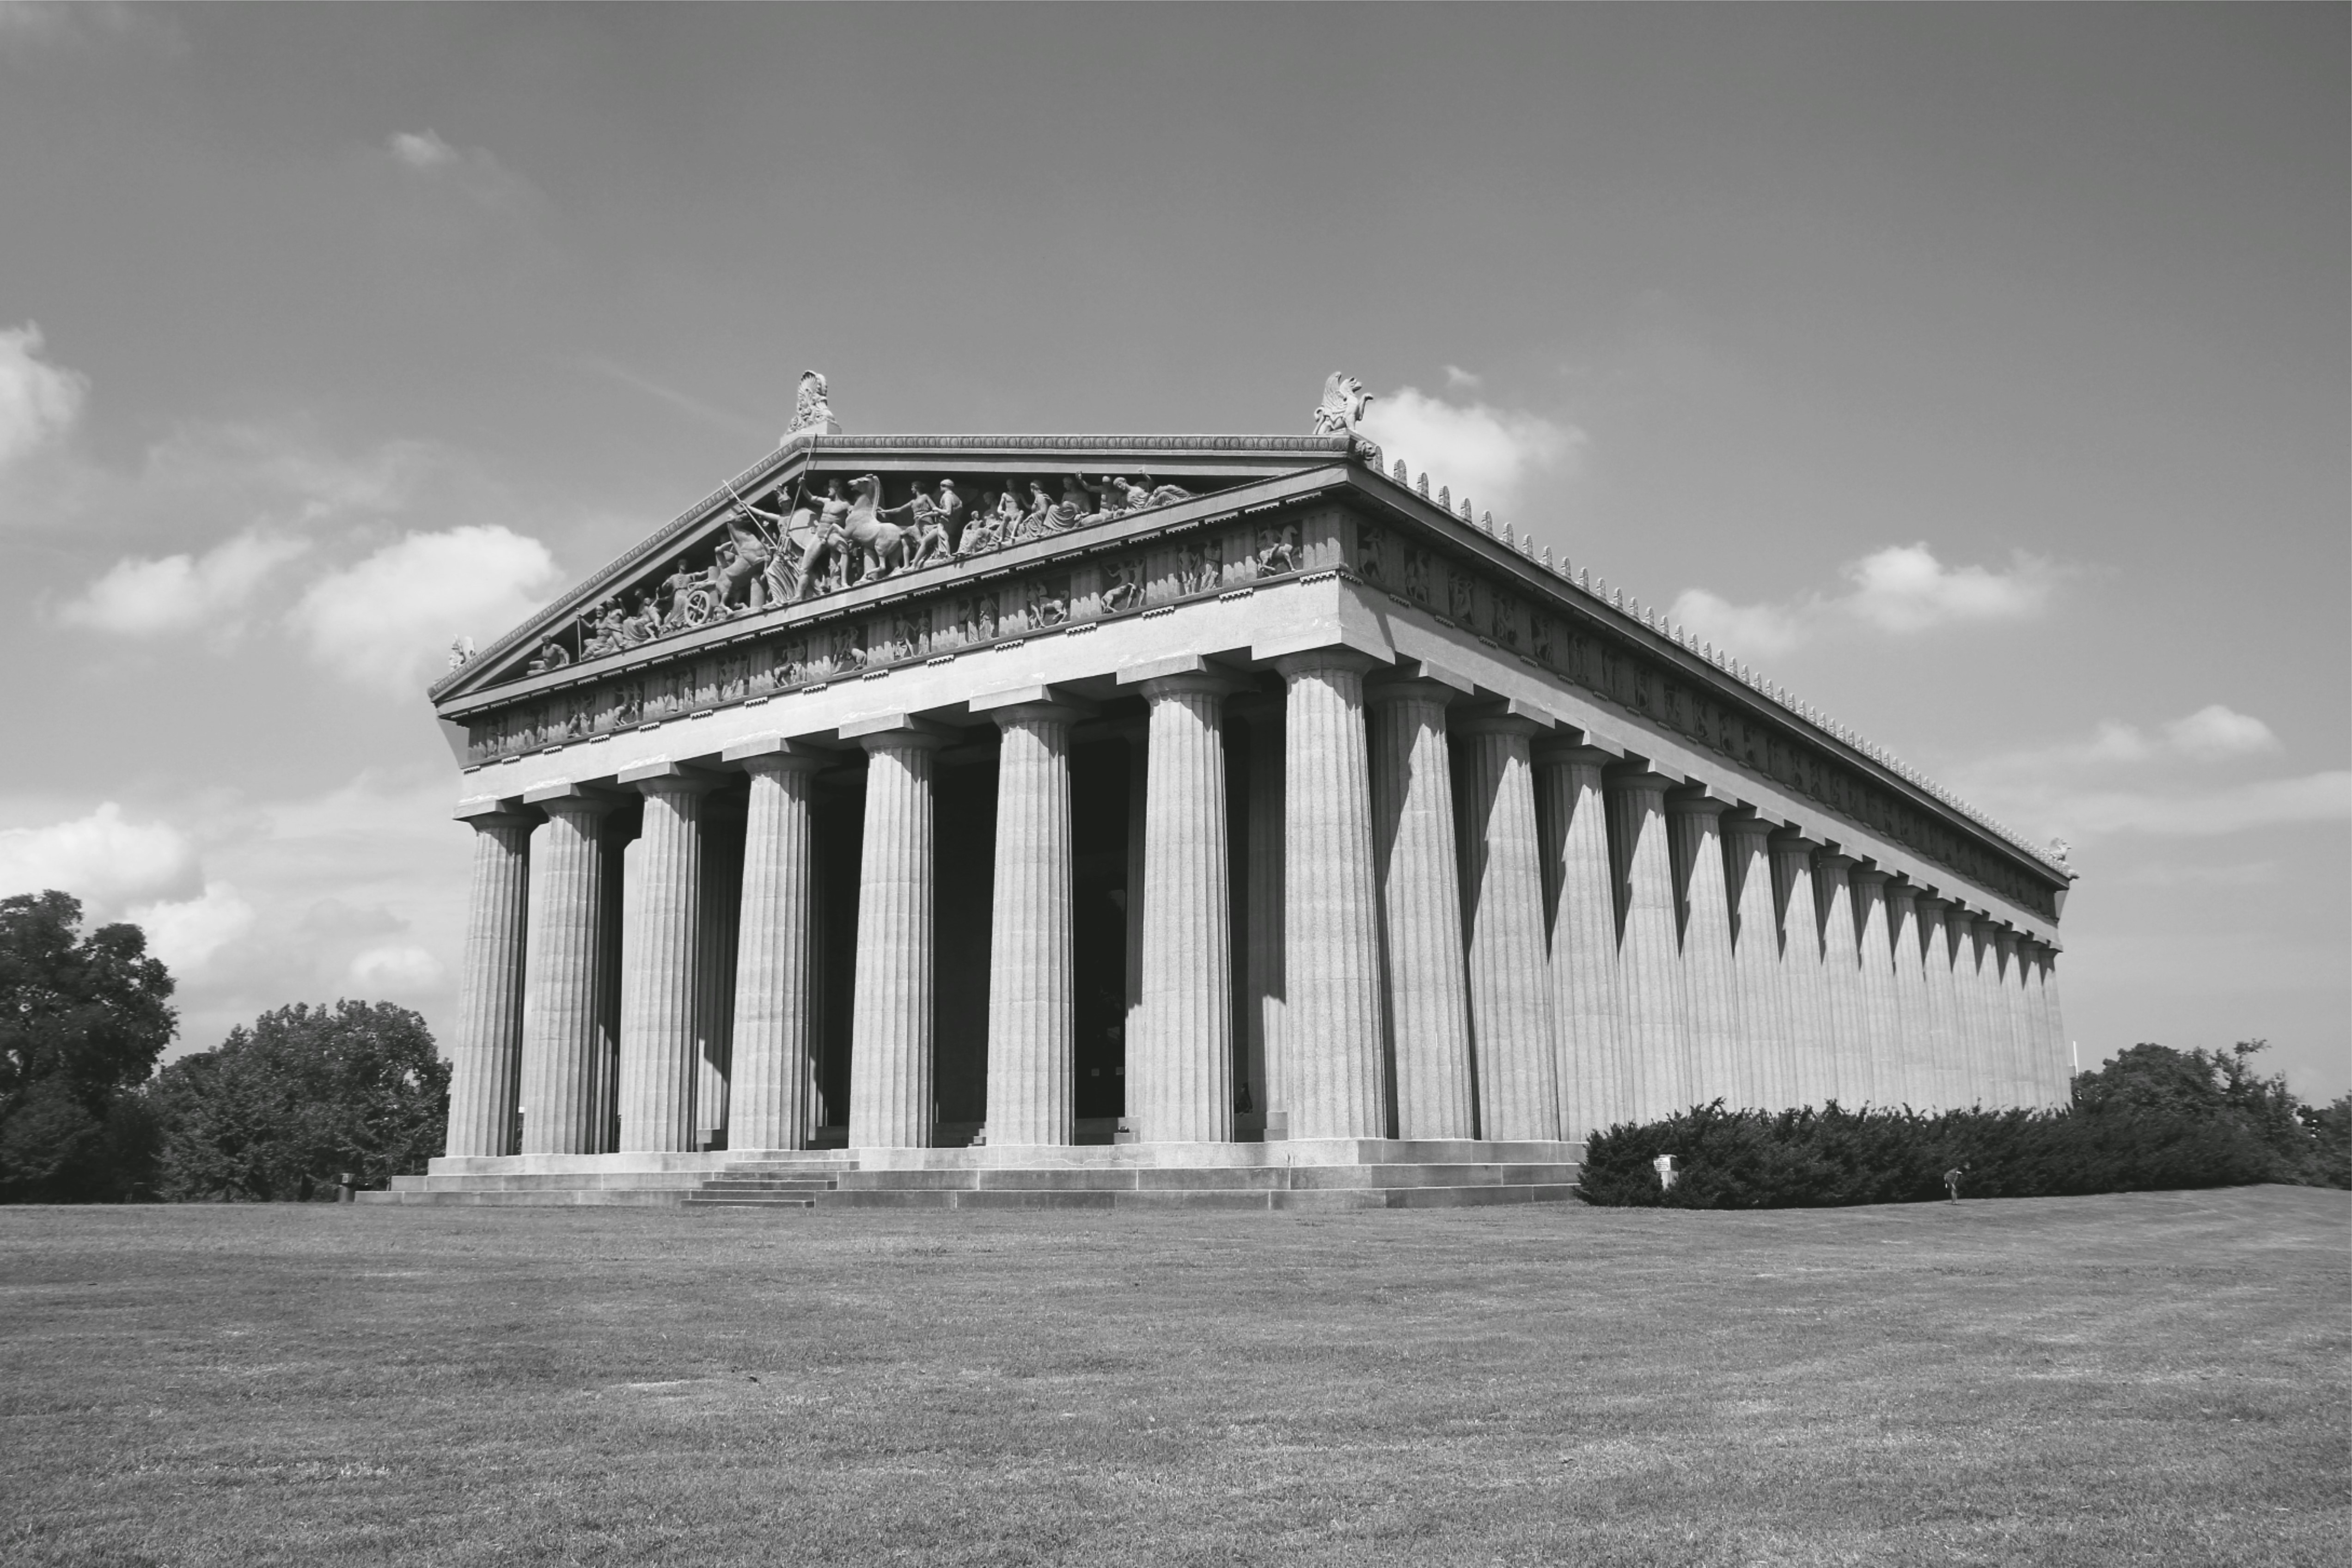
\includegraphics[width=0.7\linewidth]{images/Parthenon_Nashville_bw} 

}

\end{figure}

\newpage

\hypertarget{section:MKT}{%
\section{Mathematical Knowledge for Teaching}\label{section:MKT}}

In his presidential address to the American Educational Research Association, Lee Shulman (\citet{shulman1986}) popularized the concept of knowledge for teaching that included a specialized content knowledge where ``the teacher need not only understand \emph{that} something is so; the teacher must further understand \emph{why} it is so, on what grounds its warrant can be asserted, and under what circumstances our belief in its justification'' (p.~9). Researchers in mathematics education further expanded on this idea in the development of domains of Mathematical Knowledge for Teaching. This textbook focuses on the Subject Matter Knowledge side of the Mathematical Knowledge for Teaching.

\begin{figure}

{\centering 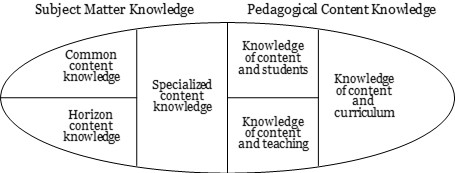
\includegraphics[width=1\linewidth]{tikz/ballegg1} 

}

\caption{Domains of Mathematical Knowledge for Teaching [@Ball2008]}\label{fig:unnamed-chunk-3}
\end{figure}

\hypertarget{common-content-knowledge}{%
\subsection{Common Content Knowledge}\label{common-content-knowledge}}

The foundation for much of the other aspects of mathematical knowledge for teaching is \textbf{common content knowledge}, defined as ``the mathematical knowledge and skill used in settings other than teaching'' \citep[p.~399]{Ball2008}. Common content knowledge provides the individual the ability to solve mathematical problems from the related curriculum and to apply the mathematical knowledge to other fields of knowledge outside of mathematics. Common content knowledge also includes understanding how some of the different mathematical subjects build upon one another, but does not require those studying the material to be able to explain broader patterns. Thus, common content knowledge represents the type of knowledge that we expect secondary and introductory post-secondary students to display.

For instance, common content knowledge related to rational algebraic expressions and functions includes understanding the relationships between rational expressions and rational numbers, how long-division of polynomials relates to long-division of integers, and the properties of the quotient and remainder of a rational expression and its effect on the graph of the related function. While this common content knowledge includes a deeper level of knowledge and a richer web of conceptual understanding by the teacher than is common for most K-12 students, the knowledge still falls within the expectations for the most advanced of these K-12 students. Thus, it is paramount that secondary mathematics teachers develop deep fluency in common content knowledge and the interconnectedness of the many different mathematical concepts in the curriculum. Such a deep and interconnected knowledge base of the teacher provides a requisite foundation in helping K-12 students learn mathematics. However, it is only a first step.

\hypertarget{specialized-content-knowledge}{%
\subsection{Specialized Content Knowledge}\label{specialized-content-knowledge}}

\textbf{Specialized content knowledge} incorporates mathematical knowledge that goes beyond knowledge expected of students, with a focus on the mathematical knowledge that improves the ability of the teacher to assist students learning mathematics \citep[p.~400]{Ball2008}. Thus, specialized content knowledge supplements the common content knowledge that all K-12 students of mathematics need. For example, while common content knowledge for rational algebraic expressions and rational functions include the relationships to the rational numbers, specialized content knowledge could include knowledge of rings and integral domains, thereby improving the teacher's ability to help students to make the connections between various pieces of related content knowledge.

A teacher would also use this specialized content knowledge related to rational expressions when explaining the extent to which two rational expressions are equivalent when common factors of the numerator and denominator cancel. For instance the teacher could explain the ways in which the expressions
\[ \frac{(x-1)(x+2)^2}{(x+1)(x+2)} \quad \mbox{and} \quad \frac{(x-1)(x+2)}{(x+1)}\] are equivalent and distinct.

\hypertarget{horizon-content-knowledge}{%
\subsection{Horizon Content Knowledge}\label{horizon-content-knowledge}}

Excellent teachers use more than just a knowledge of the content in the current curriculum when teaching students. They also draw on knowledge of what their students have previously learned in mathematics, what mathematics content will be covered in the next few years, and how the current mathematical topic relates to applications outside of mathematics. That is, excellent mathematics teachers see their instruction as part of a continuum, of which their work is only a small part. We call this domain of knowledge \textbf{horizon content knowledge}.

For example, a teacher with horizon content knowledge might use students' familiarity with rational numbers to help high school students develop knowledge of rational algebraic expressions and functions. She could also use her knowledge from differential equations to know that the rational functions play a pivotal role in the Laplace transform, helping to determine the amount of time and detail appropriate for teaching about the quotient and remainder theorem for polynomials and how to rewrite rational expressions using partial fractions. The teacher could also use knowledge of the physics curriculum and Boyle's law to help students make connections between rational expressions and functions and other fields of study. While each of these pieces of knowledge are not essential for mathematics teachers, the more knowledge one has, the better that teacher can help students learn and apply the critical components of the content.

\hypertarget{exercises}{%
\subsection{Exercises}\label{exercises}}

\begin{enumerate}
\def\labelenumi{\arabic{enumi}.}
\item
  Consider the general quadratic expression \(ax^2 + bx+c\), where \(a\), \(b\), and \(c\) are real numbers such that \(a\neq0\).

  \begin{enumerate}
  \def\labelenumii{\alph{enumii}.}
  \item
    Write a list of everything you \textbf{know} about the general quadratic expression.
  \item
    Write a list of everything you can \textbf{do} to the general quadratic expression.
  \item
    How are quadratic expressions different than quadratic equations?
  \item
    How does the factorization of a quadratic expression relate to prime numbers?
  \item
    How much do you know about the ways in which quadratic expressions are used outside of mathematics?
  \item
    Review the mathematics standards for quadratic expressions for your state. How many of the things you have listed for parts (a) and (b) match up with those standards?
  \item
    For each of your answers to a. through e., does the content you have listed or described align most with common content knowledge, specialized content knowledge, or horizon content knowledge?
  \end{enumerate}
\item
  Consider a triangle. A particular high school geometry textbook defines a triangle as ``a polygon with three sides.'' A second textbook defines a triangle as ``the figure formed by connecting three non-co-linear points with straight segments.'' A last textbook defines triangles as ``A three-sided figure.''

  \begin{enumerate}
  \def\labelenumii{\alph{enumii})}
  \item
    Are all three definitions accurate, or do some allow for shapes that might not be triangles as you understand them to be included within the category of triangle?
  \item
    In what ways might each definition be considered sloppy? That is, are there any parts of the definition that might not be well-defined? In what ways might each definition make using triangles in future lessons more difficult?
  \item
    What information do you think each textbook has presented prior to giving its definition for a triangle?
  \item
    How might horizon content knowledge help an instructor preparing a lesson on triangles decide whether a definition is appropriate or not for her students?
  \end{enumerate}
\end{enumerate}

\hypertarget{mathematical-practice-standards}{%
\section{Mathematical Practice Standards}\label{mathematical-practice-standards}}

Just like almost all of the content taught in secondary schools, the development of procedural habits and pieces of information are important parts of a secondary education, the heart of learning lies in developing habits of thinking, perseverance techniques, and developing communication skills to improve the ability to interact with the world around them. For example, the United Nations Educational, Scientific, and Cultural Organization (UNESCO) and the United Nations Office on Drugs and Crime (UNODC) \citeyearpar{UNESCO} described cognitive learning outcomes for secondary education such that a student ``Knows about local, national, and global governance and accountability systems and structures, understands issues affecting interaction and connectedness of communities at local, national and global levels, (and) develops skills for critical inquiry and analysis'' (p.~16). Mathematics, despite it's reputation, aligns well with these goals. Critical thinking, reasoning, and communicating are the most important components of the secondary mathematics curriculum, and are often the most ignored.

The National Council of Teachers of Mathematics \citeyearpar{PSSM} describes these goals in the -Principles and Standards for School Mathematics-, giving them the name `Process Standards.' The National Governors Association Center for Best Practices and the Council of Chief State School Officers \citep{CCSS} expanded upon these to create the `Common Core State Standards Standards for Mathematical Practice.' These practice standards are listed in Table \ref{tab:SMPs} and more details about these standards can be found in their corresponding publications.

\begin{table}

\caption{\label{tab:SMPs}NCTM Process Standards and  Common Core Standards for Mathematical Practice}
\centering
\begin{tabular}[t]{l|l}
\hline
Standards for Mathematical Practice & Process Standards\\
\hline
Make sense of problems and persevere in solving them. & Problem Solving\\
\hline
Reason abstractly and quantitatively. & Reasoning and Proof\\
\hline
Construct viable arguments and critique the reasoning of others. & Communication\\
\hline
Model with mathematics. & Connections\\
\hline
Use appropriate tools strategically. & Representations\\
\hline
Attend to precision & \\
\hline
Look for and make use of structure. & \\
\hline
Look for and express regularity in repeated reasoning. & \\
\hline
\end{tabular}
\end{table}

It is worth noting that these practices are expected of students of mathematics at \emph{all} grade levels. In order to help others develop these practices, we must first develop them in ourselves. Only then will we be in a position to create a learning environment that motivates and enables students to grow in these practices.

To support the users of this text in developing these practices, opportunities to practice them are woven into the text, exercises, and projects. However, as any good teacher knows, the learner needs to be actively engaged in order for an objective to be reached. As you work through the text, pay attention to how the arguments are presented and seek to understand the process behind the mathematical content. When completing the exercises and projects, do not just try to get an answer. Instead, take some time to grapple with the ideas, think of better ways to communicate what you do not understand, and seek to understand the deeper connections involved in the task.

For the purpose of this text we group these practice standards into four categories: mathematical problem solving, modeling with mathematics, communicating mathematically, and understanding mathematical structures. We briefly elaborate on each in the following sections.

\hypertarget{mathematical-problem-solving}{%
\subsection{Mathematical Problem Solving}\label{mathematical-problem-solving}}

Mathematical problem solving is perhaps the most widely cited application of mathematics ``in the real world''. Although generally acknowledge as important, problem solving is a complex process that is difficult to teach. In his book \emph{How to Solve It: A new aspect of mathematical method}, George Pólya described four phases of the problem solving process (See Figure \ref{fig:polya} when approaching mathematical problems \citep{Polya1945}. While many others have expanded on this problem solving process, much of the thinking around problem solving still traces back to the four phases that Pólya describes.

\begin{figure}

{\centering 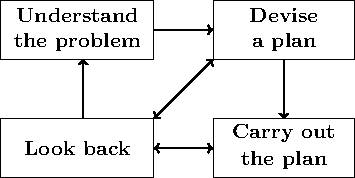
\includegraphics[width=0.45\linewidth]{tikz/polya} 

}

\caption{Pólya's problem solving process}\label{fig:polya}
\end{figure}

The first phase is the process of understanding the problem. What this phase looks like varies by problem, but often involves making sure you understand what information is given and relevant. It also includes knowledge of what an answer should look like for the question posed and, where relevant, being able to organize the provided information in a picture or diagram to better understand the situation. So, for example, if the problem is computational, understanding the problem may entail understanding whether positive or negative answers are valid solutions. If the problem is a theorem that needs proving, this phase may involve generating related examples or writing out relevant definitions to make sure you understand the given inputs and implications of the theorem.

The second phase of the problem solving process is to devise a plan. Many students struggle in the problem solving process because they only want to solve problems for which they have previously been given a template. The origin of this desire has roots in the fact that many teachers only assign students problems that are similar to those discussed in class. True mathematical problem solving involves confronting problems for which the solution is not immediately obvious to the problem solver. In problem solving, one may need to connect the current problem to previously solved problems or restate the problem in a different form with an easier solution process. Sometimes a full plan is not possible at the beginning and the solver needs to just plan initial steps and work through those to gather more information about the problem that will help them create a new plan later in the process.

Once an initial plan is devised, it needs to be carried out. This is often the simplest part of the problem solving process, and often the only component that students complete. With today's technology, computer applications can often complete the details of this part of the problem solving process through statistical analyses, computer algebra systems, or graphical programs.

After the plan is carried out, it is important to look back, completing the final phase of the problem solving process. In this step the problem solver determines whether their solution makes sense in the context of the original problem. For example, in calculus, it is often possible to obtain negative solutions that are not appropriate to the problem posed. The final step of looking back also entails making sure that we have actually addressed the question asked or the problem posed, rather than a different, somewhat related, question or problem.

Although these four phases appear linear, the majority of mathematical problems require various iterations of these phases. In particular, it is often the case that the first plan created to solve a problem does not work, so it has to be revised following an attempt to carry it out. Good problem solvers see these revisions as opportunities to learn more about the problem, rather than as failure at the problem solving process.

\hypertarget{modeling-with-mathematics}{%
\subsection{Modeling with Mathematics}\label{modeling-with-mathematics}}

Mathematical problem solving often relies on modeling with mathematics, particularly in the context of real-world phenomena. The Guidelines for Assessment and Instruction in Mathematical Modeling Education (GAIMME) defines mathematical modeling as ``a process that uses mathematics to represent, analyze, make predictions or otherwise provide insight into real-world phenomena'' \citep[p.~8]{GAIMME}. This definition varies from other common connotations of ``modeling'' that are used in education, including in mathematics. For example in mathematics education, using manipulatives to model a mathematical idea; sketching graphs or pictures to communicate or understand concepts; and demonstrating how to solve certain types of problems are all referred to as modeling. However, as a process standard, modeling mathematics does not generally include these activities. Instead, it refers to activities of using mathematics to analyze, predict, and represent real-world data.

The GAIMME Report breaks the mathematical modeling process into the six components shown in Figure \ref{fig:GAIMME}. Critically, these six components \textbf{do not} happen in a progression, but instead are iterative and sometimes run parallel to each other.

\begin{figure}

{\centering \includegraphics[width=0.7\linewidth]{tikz/GAIMME} 

}

\caption{The Math Modeling Process [@GAIMME, p. 13]}\label{fig:GAIMME}
\end{figure}

The focus on trying to better understand real-world phenomena distinguishes mathematical modeling from application problems or word problems. Actual real-world phenomena are distinctly messy and arriving at a final solution requires interpretation and assumptions. Moreover, an individual engaged in modeling has to confront the challenge of determining whether the question, mathematical model, and data are well-aligned. Teachers face the additional challenge of ensuring that the situations they create for their students are appropriate for their students. For instance, an elementary school classroom might plant some seeds in the soil. The teacher would then assist the students in identifying specific questions that can be answered quantitatively about the seeds and plants, guiding them towards a set of questions and data that the children could collect, analyze, and interpret. A secondary teacher teaching about exponential functions may introduce the class to the concept of population growth and guide the students to questions that can be answered quantitatively with exponential models. In both these examples, the instructor introduces the students to a real-world situation and then guides them to questions that facilitate the students' development of the mathematical modeling they want to discuss.

Another key aspect of the modeling process involves determining the relevance of various quantities in the situation and how to describe them with variables. This cyclical process involves identifying variables, assigning them labels and then assessing how they fit in with other variables. This process allows the modeler to create an idealized version of the original problem in order to create some type of solution. It is important during the process to justify each assumption made and to clearly label each variable, along with its appropriate units. It is through this justification process that the modeler can communicate the applicability and interpretation of the results from the model to the consumer.

As the modeler defines the variables and the relationships between them, she can use the mathematical problem solving techniques to `do the math' and come up with possible solutions to the problems posed. This section of `doing the math' reflects the word problems of most math textbooks since the word problems rarely have extraneous information and have obvious variables defined with transparent relationships between them.

Similar to the `looking back' phase of the mathematical problem solving process, the modeling process includes a stage during which the modeler steps back and assesses the model. During this stage he or she analyzes and tests the model and solution, examining the model created and determining the appropriateness and accuracy of the solution produced. This process often results in a revision to the original assumptions and adjustments to the model with improved variables and relationships between the variables.

Since the mathematical modeling process deals with messy real-world phenomena, an iterative process of reflection that results in the refinement and, where appropriate, extension, of the the model is a key component that almost always appears in a modeling cycle. This process may run parallel to or between any of the other phases of the modeling process.

When the model gets to a state that satisfies the modeler in terms of the model justifications and appropriateness of the solutions, the implementation of the model and the reporting of the results occurs. The presentation of the results must include the justification for the model, a description of the various assumptions made to produce the model, and any limitations the model has in terms of the accuracy of the results. This presentation must be done in a way that is comprehensible to the desired audience. Because modeling deals with real-world situations, the solution is unlikely to be clear or definitive, but will instead be approximate and estimated.

\hypertarget{communicating-mathematically}{%
\subsection{Communicating Mathematically}\label{communicating-mathematically}}

Mathematical communication broadly relates to the ways and methods of representing, justifying, and interpreting mathematics. More specifically, the practice of mathematical communication ``encompasses both listening and reading (comprehension) and both speaking and writing (expression)\ldots{} and may also include representation of mathematical ideas in nonlinguistic ways'' \citep[p.~7]{Communication}. In order to better understand the practice of communicating mathematically, we examine six overlapping concepts that are at the core of this practice (see Figure \ref{fig:communication}).

\begin{figure}

{\centering 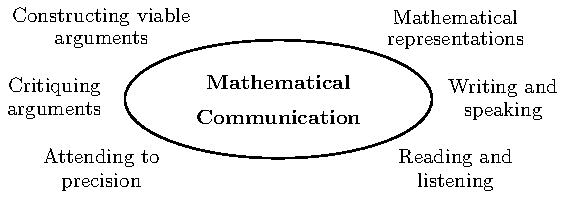
\includegraphics[width=0.6\linewidth]{tikz/communication} 

}

\caption{Components of Mathematical Communication}\label{fig:communication}
\end{figure}

All types of communication require a language. Within a language there exists a shared meaning behind the words and symbols used when communicating with a particular language. Mathematics communication, in this sense, operates much as a language does. However, unlike a language such as English, mathematics is represented using a mixture of words that have very precise definitions and symbols that compress many different ideas and meanings into a very small amount of space (linguists call mathematics a ``dense'' language because of this property). Moreover, somewhat uniquely to mathematics, the meaning of symbols varies widely depending upon the context of the communication. Consider variables, which are usually represented using any number of symbols. While certain types of symbols will cue a well-informed mathematics student that a variable has some implied meaning in terms of what type of number system to which it belongs, even in this case variables in different circumstances serve different roles. Sometimes the letter represents a fixed value (e.g., \(x=4\)) and other times it represents a range of values that satisfy a particular condition (e.g., \(x\leq 4\)). Sometimes it indexes a set, while other times it represents a function. The differences between these uses are often subtle, making explicit training in these nuances mathematics critical.

Once the language of mathematics has been developed, the grammar is created. In mathematics, logic, argument, and proof form the core patterns of organization and presentation. Together, logic, argument, and proof boil down to the ability to construct viable arguments and critique the arguments of others using mathematical evidence.

Part of mathematical communication is learning how to consume and understand the ideas of others. In mathematics this usually occurs by reading or listening to the arguments of others. Both reading and listening to mathematics require a great deal of practice and are skills students must hone over many courses. In particular, reading mathematics requires a great deal of practice and discipline. While a novel can usually be consumed at a steady pace without much explicit effort by the reader, written mathematical ideas are often presented symbolically, with the reader left to fill in certain logical steps. Thus, the act of reading mathematics becomes one of translation of the symbolic work into a language he or she understands, followed by a effort to connect current parts of the argument to previously made points, and the absorption and evaluation of those ideas based on previous knowledge. As a result, reading mathematical texts and arguments requires a big investment in time. Sometimes it can take hours just to understand one line of a mathematical text! This slow, methodical way of reading is challenging to students of mathematics, but is a critical skill to develop as it is core to the practice of doing mathematics.

Previous paragraphs have described the difficulties and process of consuming mathematical texts. However, it is also important that students learn to produce their own mathematical communications in both oral and written forms. In communicating to others, it is essential that precise mathematical words are used, rather than slang, in order to reduce the confusion of potential readers. It is also useful to employ a variety of mathematical representations, including graphs, sketches, and diagrams to facilitate the communication of mathematical ideas.

As teachers of mathematics, we must continually emphasize the development of this practice of communicating mathematically by de-emphasizing simple answers to mathematical problems, teaching students how to read and write mathematics (not just about mathematics), and to promote classroom discourse to provide opportunities for students to experience different types of mathematical communication.

\hypertarget{understanding-mathematical-structures}{%
\subsection{Understanding Mathematical Structures}\label{understanding-mathematical-structures}}

While the definition of mathematics is not uniform or agreed on, most agree that mathematics is inherently about the study of underlying structures and logical reasoning. For example, the Encyclopædia Britannica \citeyearpar{definition} defines mathematics as ``the science of structure, order, and relation that has evolved from elemental practices of counting, measuring, and describing the shapes of objects.'' This means that an important practice in the doing of mathematics is to ``look for and make use of structure'' and to ``look for and express regularity in repeated reasoning'' \citep{CCSS}.

The pursuit and use of structure and regularity appear throughout all of mathematics. Mathematical structure informs every part of mathematics teaching, from instruction on common mathematical procedures to searching for and making connections between various, apparently unrelated, mathematical content areas to provide new insight into a problem. As teachers, we need to point out these mathematical structures to the students and help them learn how to discover the structures and regularity on their own.

\hypertarget{exercises-1}{%
\subsection{Exercises}\label{exercises-1}}

\begin{enumerate}
\def\labelenumi{\arabic{enumi}.}
\item
  Consider the following mathematical task:

  An electricity company charges Kelly \(\$0.15\) per kWh (kilowatt-hour) of electricity used, plus a basic connection charge of \(\$8.00\) per month. Find a function that helps Kelly estimate her monthly electricity bill for a given number of kWhs. Be explicit about the domain of the function you create.

  \begin{enumerate}
  \def\labelenumii{\alph{enumii})}
  \item
    NCTM emphasizes multiple representation of functions using verbal, tabular, graphical, and symbolic representations. Using this word problem as the verbal representation, express the function in each of the remaining ways.
  \item
    How does the ability to move between different representations of functions support students' development of the mathematical communication process standard?
  \item
    The problem solving section discussed the fact that a mathematical task is only considered a problem if the person working on the task does not know in advance a solution method that will produce a correct answer. Would you say that for part (a) you were engaged in mathematical problem solving as described in the standards? Why or why not?
  \item
    Under what conditions would the task be a problem for students you were teaching?
  \item
    Based on the description of mathematical modeling, would you say that finding the function for the task in part (a) represents mathematical modeling? Why or why not?
  \item
    A second part of the task asks students to estimate Kelly's electrical bill for the year, given that her monthly kWh usage ranges between 202 and 254 kWh.
  \item
    The textbook you got the problem from lists the answer to the extension as \(\$506.40\). What did the author do and what assumptions did she make in order to arrive at that answer? Do you agree with her process and assumptions? Why or why not?
  \item
    In arriving at your answer for part (a), would you say that you were engaged in mathematical problem solving? Why or why not?
  \item
    If you were using this task as a modeling activity for your students, what criteria would you use to evaluate whether their answer was reasonable?
  \end{enumerate}
\item
  There are five NCTM Process Standards and eight Common Core Standards for Mathematical Practice. While there is significant overlap between the two sets of standards, they are not the same. Read each set of standards. When there is overlap between the two sets of standards, create a map between them. Also identify the ways in which the two sets of standards differ. These regions are not at the heading level. You'll have to actually dig into the blurbs about each standard in their original documents.
\item
  A basic theorem that students use from an early age is that the sum of two even integers is even. A typical proof of this theorem might look something like this:

  Let \(a\) and \(b\) be even integers such that \(a=2m\) and \(b=2n\) where \(m\) and \(n\) are integers. Then \(a+b=2m+2n=2(m+n)\). Thus, the sum of two even integers is even.

  \begin{enumerate}
  \def\labelenumii{\alph{enumii})}
  \item
    The section on mathematical communication emphasizes the reliance of mathematical communication on precise definitions and symbols that compress complex ideas into short phrases. In examining this proof, identify the places where the problem statement or proof rely on a definition or compressed expression.
  \item
    Identify the places where the proof writer has left the reader to fill in logical steps or rationales.
  \item
    Rewrite the proof of the theorem without the use of any symbols, but with the same degree of precision and generalizability.
  \item
    In comparing the symbolic proof to your verbal proof, do you think it is easier to understand (i.e., more like a novel?) or do you think it would still be difficult to read if all mathematics were presented without symbols? Why or why not?
  \item
    If you reflect on the six parts of mathematical communication, which parts do you think you are best at? Which parts do you struggle the most with? What is one goal you have for yourself for mathematical communication that you want to develop during this course?
  \end{enumerate}
\end{enumerate}

\hypertarget{mathematics-content-standards-in-the-u.s.}{%
\section{Mathematics Content Standards in the U.S.}\label{mathematics-content-standards-in-the-u.s.}}

The current standards for mathematics and assessment in the United States are derived from a variety of sources and past initiatives. David Klein \citeyearpar{Klein2003} gives a good summary of the major events and influential individuals during the 20\textsuperscript{th} century. The current set of standards have origins to a pair of reports from the 1980's: one by NCTM \citeyearpar{NCTM1980}, \emph{An Agenda for Action}, and one by the U.S. National Commission on Excellence in Education \citeyearpar{NCEE1983}, \emph{A Nation at Risk}. Each provided a different view about what should occur to improve mathematics education in the United States. While these two documents were used as the basis for the `math wars' of the late 20\textsuperscript{th} century, the biggest difference between them is that the NCTM document focused primarily on standards for teaching methodologies, while \emph{A Nation at Risk} focused on standards of content knowledge.

The NCTM \citeyearpar{NCTM1980} recommended "that

\begin{enumerate}
\def\labelenumi{\arabic{enumi}.}
\item
  problem solving be the focus of school mathematics in the 1980s;
\item
  basic skills in mathematics be defined to encompass more than computational facility;
\item
  mathematics programs take full advantage of the power of calculators and computers at all grade levels;
\item
  stringent standards of both effectiveness and efficiency be applied to the teaching of mathematics;
\item
  the success of mathematics programs and student learning be evaluated by a wider range of measures than conventional testing;
\item
  more mathematics study be required for all students and a flexible curriculum with a greater range of options be designed to accommodate the diverse needs of the student population;
\item
  mathematics teachers demand of themselves and their colleagues a high level of professionalism;
\item
  public support for mathematics instruction be raised to a level commensurate with the importance of mathematical understanding to individuals and society" (p.~1).
\end{enumerate}

The National Commission on Excellence in Education \citeyearpar{NCEE1983} recommended that

\begin{itemize}
\item
  ``The teaching of \emph{mathematics} in high school should equip graduates to: (a) understand geometric and algebraic concepts; (b) understand elementary probability and statistics; (c) apply mathematics in everyday situations; and (d) estimate, approximate, measure, and test the accuracy of their calculations. In addition to the traditional sequence of studies available for college-bound students, new, equally demanding mathematics curricula need to be developed for those who do not plan to continue their formal education immediately'' (p.~25).
\item
  ``Standardized tests of achievement (not to be confused with aptitude tests) should be administered at major transition points from one level of schooling to another and particularly from high school to college or work. The purposes of these tests would be to: (a) certify the student's credentials; (b) identify the need for remedial intervention; and (c) identify the opportunity for advanced or accelerated work. The tests should be administered as part of a nationwide (but not Federal) system of State and local standardized tests. This system should include other diagnostic procedures that assist teachers and students to evaluate student progress'' (p.~28).
\item
  ``Persons preparing to teach should be required to meet high educational standards, to demonstrate an aptitude for teaching, and to demonstrate competence in an academic discipline. Colleges and universities offering teacher preparation programs should be judged by how well their graduates meet these criteria'' (p.~30).
\item
  ``Substantial nonschool personnel resources should be employed to help solve the immediate problem of the shortage of mathematics and science teachers. Qualified individuals including recent graduates with mathematics and science degrees, graduate students, and industrial and retired scientists could, with appropriate preparation, immediately begin teaching in these fields. A number of our leading science centers have the capacity to begin educating and retraining teachers immediately. Other areas of critical teacher need, such as English, must also be/addressed'' (p.~31).
\end{itemize}

NCTM followed it's 1980 report with the publication of the \textit{Curriculum and Evaluation Standards for School Mathematics} \citep{NCTM1989}. This document focused on the standards for teaching methodologies and mathematical practices. Content standards were sketched out, with overviews of the recommended content knowledge for students in 4-year grade bands. NCTM expanded this work with additional texts focusing on teaching standards and assessment: \textit{Professional Teaching Standards} (\citeyear{NCTM1991}) and \textit{Assessment Standards} (\citeyear{NCTM1995}). In 2000, NCTM released an updated version the 1989 standards with the \textit{Principles and Standards for School Mathematics} \citep{PSSM}. During this same time, many states developed more specific content standards reflecting the guidelines recommended by the 1989 document \citep{Raimi1998}. Although the NCTM document did not make content recomendations by specific grade levels, many of the state standards still resided at the grade-band level \citep[p. 677]{Reys2007}.

\hypertarget{common-core-state-standards-math}{%
\subsection{Common Core State Standards-Math}\label{common-core-state-standards-math}}

In 2002, Congress passed the No Child Left Behind Legislation. This bill required that states determine measurable content standards for each grade level and develop assessments based on these standards to be given to all students at specific grade levels (generally fourth, eighth, and twelfth grade) in order to receive federal school funding. Since each state developed their own standards, the level and specificity of these standards varied greatly between States \citep{Reys2007}.

It was in this environment that the National Governors Association Center for Best Practices and the Council of Chief State School Officers launched an effort in 2009 to develop ``a common core of internationally benchmarked standards in math and language arts for grades K-12'' \citep{CCSS}. These standards emphasize content knowledge, while also encouraging some of the teaching methodologies proposed by the NCTM documents.

In order to help teachers better understand how the topics in this book relate to the actual teaching and learning of their students, we include related content standards from the Common Core State Standards for Mathematics throughout the text. While not all states have adopted the Common Core State Standards for their school systems, these standards are a good representation of what is expected from students at different stages in their mathematical education.

\begin{quote}
\hypertarget{related-content-standards}{%
\subsubsection*{Related Content Standards}\label{related-content-standards}}
\addcontentsline{toc}{subsubsection}{Related Content Standards}

\begin{itemize}
\tightlist
\item
  (8.F.1) Understand that a function is a rule that assigns to each input exactly one output. The graph of a function is the set of ordered pairs consisting of an input and the corresponding output.
\item
  (HSF.IF.7) Graph functions expressed symbolically and show key features of the graph, by hand in simple cases and using technology for more complicated cases.
\end{itemize}
\end{quote}

Standards that align with the content of each section are provided in blocks with the title ``Related Content Standards.'' One such box is given above as an example. The sequence of numbers and letters proceeding each standard is its standardized abbreviation. The first part of the abbreviation identifies the grade band. Since the Common Core State Standards for high school do not have a recommended grade level for each of the standards, they are denoted by ``HS'' and the general area of mathematics. The second part of the abbreviation refers to the general domain of mathematics, and the third part refers to the location of the standard in that grade band and domain.

\hypertarget{nctm-caep-standards}{%
\subsection{NCTM-CAEP Standards}\label{nctm-caep-standards}}

Another requirement of the No Child Left Behind legislation was that states had to create standards for teachers to receive certification. These standards for certification needed to be measured with a blend of standardized assessments, portfolios, and coursework. As a result, certification in secondary mathematics in most states requires a major in mathematics (or its equivalent), the teaching of and about standards during certification coursework, and achievement of certain scores on a content specific standardized test (such as the PRAXIS). In addition, the NCTM partnered with the Council for the Accreditation of Educator Preparation (CAEP) to develop standards for what beginning secondary mathematics teachers should know and be able to do in the teaching of mathematics \citep{CAEP}.

The NCTM-CAEP content standards are built upon the standards developed by the Conference Board of Mathematical Sciences in \citeyearpar{MET1} and \citeyearpar{MET2}. The content of this book builds upon the contents of the first standard of ``Knowing and Understanding Mathematics''. In particular:

\begin{quote}
Candidates demonstrate and apply, with the incorporation of mathematics technology, conceptual understanding, procedural fluency, and factual knowledge of major mathematical domains: Number; Algebra and Functions; Statistics and Probability; Geometry, Trigonometry, and Measurement; Calculus; and Discrete Mathematics.
\end{quote}

We list the details of the NCTM-CAEP content standards below and discuss how this book connects to each of these standards.

\begin{quote}
\textbf{Essential Concepts in Number.} Candidates demonstrate and apply conceptual understanding, procedural fluency, and factual knowledge of number including flexibly applying procedures, using real and rational numbers in contexts, developing solution strategies, and evaluating the correctness of conclusions. Major mathematical concepts in Number include number theory; ratio, rate, and proportion; and structure, relationships, operations, and representations.
\end{quote}

Number systems are primarily covered in Chapters \ref{ch:number}, \ref{ch:group-1}, and \ref{ch:rings}. We introduce initial concepts of the number systems in Chapter \ref{ch:number}, focusing on operations and the basic properties of common number systems, including whole numbers, integers, rational, real, and complex numbers. Chapters \ref{ch:group-1} and \ref{ch:rings} expand these ideas through the added structure of rings and fields.

\begin{quote}
\textbf{Essential Concepts in Algebra and Functions.} Candidates demonstrate and apply understandings of major mathematics concepts, procedures, knowledge, and applications of algebra and functions including how mathematics can be used systematically to represent patterns and relationships including proportional reasoning, to analyze change, and to model everyday events and problems of life and society. Essential Concepts in Algebra and Functions include algebra that connects mathematical structure to symbolic, graphical, and tabular descriptions; connecting algebra to functions; and developing families of functions as a fundamental concept of mathematics. Additional Concepts should include algebra from a more theoretical approach including relationship between structures (e.g., groups, rings, and fields) as well as formal structures for number systems and numerical and symbolic calculations.
\end{quote}

Many of these concepts are spread throughout the text, as algebra and functions are fundamental to the secondary curriculum. That said, Chapters \ref{ch:function}, \ref{ch:group-1}, \ref{ch:rings}, and \ref{ch:real-valued-functions} specifically focus on topics of particular importance in understanding algebra and functions. In particular Chapter \ref{ch:real-valued-functions} combines the themes of the earlier chapters together using real-valued functions.

\begin{quote}
\textbf{Essential Concepts in Calculus.} Candidates demonstrate and apply understandings of major mathematics concepts, procedures, knowledge, and applications of calculus including the mathematical study of the calculation of instantaneous rates of change and the summation of infinitely many small factors to determine some whole. Essential Concepts in Calculus include limits; continuity; the Fundamental Theorem of Calculus; and the meaning and techniques of differentiation and integration.
\end{quote}

The essential concepts in calculus are currently excluded from this text with the understanding that most pre-service teachers are already required to take at least two semesters worth of calculus courses that focus on this content standard.

\begin{quote}
\textbf{Essential Concepts in Statistics and Probability.} Candidates demonstrate and apply understandings of statistical thinking and the major concepts, procedures, knowledge, and applications of statistics and probability including how statistical problem solving and decision making depend on understanding, explaining, and quantifying the variability in a set of data to make decisions. They understand the role of randomization and chance in determining the probability of events. Essential Concepts in Statistics and Probability include quantitative literacy; visualizing and summarizing data; statistical inference; probability; and applied problems.
\end{quote}

The essential concepts of statistics and probability are the focus of Part IV of the text, Data Analysis. In that section we focus on statistics and a study of variability, looking at different ways to measure, communicate, and understand variability in the context of statistical problems.

\begin{quote}
\textbf{Essential Concepts in Geometry, Trigonometry, and Measurement.} Candidates demonstrate and apply understandings of major mathematics concepts, procedures, knowledge, and applications of geometry including using visual representations for numerical functions and relations, data and statistics, and networks, to provide a lens for solving problems in the physical world. Essential Concepts in Geometry, Trigonometry, and Measurement include transformations; geometric arguments; reasoning and proof; applied problems; and non-Euclidean geometries.
\end{quote}

Part III on Geometry looks at the subject of Geometry from the perspectives of constructional, transformational, analytic, and algebraic. Each perspective helps us to better understand the essential concepts in geometry, trigonometry, and measurement, along with the interactions between geometry, algebra, functions, and number systems.

\hypertarget{exercises-2}{%
\subsection{Exercises}\label{exercises-2}}

\begin{enumerate}
\def\labelenumi{\arabic{enumi}.}
\item
  Reflect on your K-12 mathematics education. Based on the brief history described, what documents were being used to guide your curriculum?
\item
  Those who study mathematics curriculum describe the changing focus of what is written in school standards for mathematics as a pendulum. Over time, the pendulum swings between a focus on procedural fluency such as \emph{A Nation at Risk} \citeyearpar{NCEE1983} describes and the more process oriented standards as outlined by NCTM (1989).

  \begin{enumerate}
  \def\labelenumii{\alph{enumii})}
  \tightlist
  \item
    How does the Common Core State Standards attempt to unify the two extremes of the pendulum swing?
  \item
    How does treating the process standards as separate from the content standards provide an opportunity to continue to let the pendulum swing?
  \item
    Regardless of which documents were currently in vogue while you were in school, do you think your mathematics education was more procedurally focused or more process standard focused?
  \item
    Is how you were taught what you hope your own teaching will be like? Why or why not?
  \item
    K-12 mathematics students often think that mathematics is a set of unrelated procedures that they have to memorize how to do. In contrast, people who do mathematics for a living think mathematics is a conceptual and logical system where everything fits together. As you currently understand them, do you think the Common Core State Standards could support students in moving from thinking about mathematics as a set of unrelated procedures to a more conceptual system? Why or why not?
  \end{enumerate}
\end{enumerate}

\hypertarget{ch:sets}{%
\chapter{Set Theory}\label{ch:sets}}

In the mid-1800s the field of mathematics went through a major shift that ended up changing the very definition of mathematics. In 1847, George Boole wrote in the introduction to \emph{The Mathematical Analysis of Logic} that up to that point, ``the abstractions of the modern Analysis, not less than the ostensive diagrams of the ancient Geometry, have encouraged the notion, that Mathematics are essentially, as well as actually, the Science of Magnitude'' \citep{Boole}. Instead, Boole proposed a new definition, suggesting

\begin{quote}
We might justly assign it as the definitive character of a true Calculus, that it is a method resting upon the employment of Symbols, whose laws of combination are known and general, and whose results admit of a consistent interpretation\ldots{} It is upon the foundation of this general principle, that I purpose to establish the Calculus of Logic, and that I claim for it a place among the acknowledged forms of Mathematical Analysis, regardless that in its object and in its instruments it must at present stand alone.
\end{quote}

\begin{figure}

{\centering \includegraphics[width=0.35\linewidth]{images/Portrait_of_George_Boole} 

}

\caption{George Boole}\label{fig:unnamed-chunk-4}
\end{figure}

At the time that Boole wrote the above passage, mathematics as a field shifted from the study of quantities to the study of abstract structures based on logic and set theory. This change in the definition of mathematics freed up those who studied it to move beyond structures tied to physical interpretations and applications and move to a more abstract field. The abstractification of mathematics was a powerful moment, resulting in the development of fields such as quantum mechanics, relativity, cryptography, statistics.

In this chapter we will go through some of the basics of set theory needed to understand some of the later material and to develop a common vocabulary and set of notations. We do not offer a deep treatment of set theory as there are many textbooks, specifically in the area of Discrete Math, with a more detailed coverage of it.

\hypertarget{sets-and-subsets}{%
\section{Sets and Subsets}\label{sets-and-subsets}}

The foundation of modern mathematics is the theory of sets. Informally, sets can be thought of as collections of objects. While \textbf{set theory} is not specifically outlined in the content standards of most states, it is mentioned in the Common Core standards. The first reference to set theory occurs in the Introduction to Kindergarten, stating:

\begin{quote}
Students use numbers, including written numerals, to represent quantities and to solve quantitative problems, such as counting objects in a set; counting out a given number of objects; comparing sets or numerals; and modeling simple joining and separating situations with sets of objects, or eventually with equations such as \(5 + 2 = 7\) and \(7 - 2 = 5\). (Kindergarten students should see addition and subtraction equations, and student writing of equations in kindergarten is encouraged, but it is not required.) Students choose, combine, and apply effective strategies for answering quantitative questions, including quickly recognizing the cardinalities of small sets of objects, counting and producing sets of given sizes, counting the number of objects in combined sets, or counting the number of objects that remain in a set after some are taken away. \citep{CCSS}
\end{quote}

Set theory also makes an appearance in the high school standards related to counting and probability, as knowledge of sets is critical to understanding basic formulas in probability.

\begin{quote}
\hypertarget{related-content-standards-1}{%
\subsubsection*{Related Content Standards}\label{related-content-standards-1}}
\addcontentsline{toc}{subsubsection}{Related Content Standards}

\begin{itemize}
\tightlist
\item
  (HSS.CP.1) Describe events as subsets of a sample space (the set of outcomes) using characteristics (or categories) of the outcomes, or as unions, intersections, or complements of other events (``or,'' ``and,'' ``not'').
\end{itemize}
\end{quote}

We start our exploration of set theory by developing some basic notation and definitions. \citet{Cantor} defined sets in the following way.

\begin{quote}
Unter einer `Menge' verstehen wir jede Zusammenfassung \(M\) von bestimmten wohlunterschiedenen Objecten \(m\) unsrer Anschauung oder unseres Denkens (welche die `Elemente' von \(M\) genannt werden) zu einem Ganzen. (p.~481)

By a `Set' we mean each collection \(M\) of certain well-differentiated objects \(m\) of our perception or our thinking (which are called the `elements' of \(M\)) as a whole. (English translation)
\end{quote}

This definition proved to not be precise enough to avoid certain paradoxes.

\begin{example}[Russell's Paradox]
\protect\hypertarget{exm:unnamed-chunk-5}{}{\label{exm:unnamed-chunk-5} \iffalse (Russell's Paradox) \fi{} } Let \(R= \left\{ x \middle \vert x\notin x\right\}\), the set that contains all sets that are not members of themselves. Is \(R\) an element of \(R\)? If it is, then it is a set that is an element of itself and so could not be an element of \(R\), by its definition, thus leading to a contradiction. On the other hand, if one assumes that \(R\) is not an element of itself, then it satisfies the conditions of being an element of \(R\), also leading to a contradiction. Thus defining the paradox.
\end{example}

Even though Cantor's definition of a set leads to such paradoxes, we will use it as our working definition, with the detailed definition of set being a primitive notion in Zermelo-Fraenkel set theory. The Zermelo-Fraenkel axioms, combined with the axiom of choice, create the ZFC axioms upon which mathematics is built. Due to the level of abstraction involved in the axioms, we will not include a systematic coverage of the axioms in this text, but will reference them as needed.

\begin{definition}
\protect\hypertarget{def:unnamed-chunk-6}{}{\label{def:unnamed-chunk-6} }

\begin{itemize}
\item
  We will define a set by the collection of elements which belong to the set.
\item
  If \(A\) is a set and \(a\) is an object that belongs to \(A\), we say that \(a\) is an \textbf{element} of \(A\) and denote it as \(a\in A\).
\item
  If an object \(a\) is not an element of a set \(A\), we denote that by \(a \notin A\).
\item
  Let \(A\) and \(B\) be sets. We say that \(A=B\) if and only if every element of \(A\) is an element of \(B\) and every element of \(B\) is an element of \(A\). (In the ZFC axioms, this is referred to as the axiom of extensionality.)
\end{itemize}
\end{definition}

While the elements of a set are often written in a specific order, i.e.~\(\{1,2,3\}\), the members of a set have no particular order and the same set could be written as \(\{3, 1, 2, 1\}\), with the repetition being irrelevant since the set is defined by its elements.

We also need to note that \(a\) and \(\{a\}\) are two different mathematical objects (one is the element \(a\) and the other is the set that contains the element \(a\)). So \(A = \{a, \{a\}\}\) defines a set with two distinct elements: \(a\) and \(\{a\}\). Likewise, if \(B=\{1, 2, 3, \{4\}, 5\}\), then \(4\notin B\) but \(\{4\}\in B\). So the symbol \(4\) is not an element of \(B\), but the symbol \(\{4\}\) (the set that contains the element \(4\)) does belong to \(B\). These nuances mean that we have to be very careful with our notation and how we read the mathematical symbols.

Another way to describe sets is using set-builder notation. In this notation, we describe our new set using larger sets and a set of restrictions on (or description of) which objects in the larger set we are choosing to include. For instance, we can define \(C\) to be the set of all real numbers (denoted \(\mathbb{R}\)) greater than or equal to \(3\). In this case, the larger set is the set of real numbers and the condition that the numbers are greater than or equal to three is the restriction or description. Of course we do not want to have to keep writing so much down, so we create a short-hand way of defining this set:
\[ C = \left\{ x\in \mathbb{R} \middle \vert x\geq 3\right\}\] where the \(\vert\) separates the description of the larger set and the description of the restrictions. This notation is read ``\(C\) is the set of all of the elements \(x\) in the real numbers such that \(x\) is greater than or equal to 3.'' This set-builder notation is particularly useful when describing sets with more than just a few elements.

When sets are subsets of the real numbers, we can also describe them using interval notation. For the set \(C\) defined above, we can also write
\[C=[3,\infty)\] where the closed bracket, \([\), denotes that the endpoint is contained in the set, while an open bracket, \((\), denotes that the endpoint is not contained in the set. For real numbers \(a\) and \(b\), with \(a<b\), we have the following options as intervals from \(a\) to \(b\):
\[ (a,b) \quad (a,b] \quad [a,b) \quad [a,b] .\]

Once we have created notation for sets with a few elements and a large number of elements, we can describe how to denote a set without any elements.

\begin{definition}
\protect\hypertarget{def:unnamed-chunk-7}{}{\label{def:unnamed-chunk-7} } The set that does not contain any elements is called the \textbf{empty set} and is denoted by \(\emptyset\). Any set that contains at least one element is then called \textbf{non-empty}.
\end{definition}

In addition to determining how to describe sets, we must have a way to determine if two sets are the same or distinct.

A direct consequence of this definition is that the number of times an element is listed and the order of the elements is irrelevant for equality of sets. So \(\{a, b, c, d\}=\{b, a, c, c, d, b\}\) and \(\{1, 2\} \neq \{1, 2, 3\}\).

\begin{definition}
\protect\hypertarget{def:subset}{}{\label{def:subset} } Let \(A\) and \(B\) be sets. We say that \(A\) is a subset of \(B\), denoted \(A \subseteq B\), if every element of \(A\) is also an element of \(B\). If \(A\) is not a subset of \(B\), we sometimes denote this by \(A\nsubseteq B\). If there are elements of \(A\) is a subset of \(B\) and there are elements of \(B\) that are not contained in \(A\), then we say that \(A\) is a \textbf{proper subset} of \(B\) and denote it by \(A\subset B\).
\end{definition}

For example:
\[\{6, 7 \} \subseteq \{5, 6, 7, 8\},\]
\[\{x\in \mathbb{R} \vert x>5\} \subseteq \{x\in \mathbb{R} \vert x \geq 2\}, \mbox{ and }\]
\[ \{a,b,c\} \subseteq \{a,b,c\}. \]
Notice that the first two examples are proper subsets.

It is important to distinguish between the phrases `element of' and `contained in' when discussing sets. If \(A= \{a,b,c\}\), then we say that \(a\) is an element of \(A\), while \(\{a\}\) is contained in \(A\)

Since the empty set has no elements, it is by default a subset of every set. Similarly, every set is a subset of itself.

\begin{example}
\protect\hypertarget{exm:unnamed-chunk-8}{}{\label{exm:unnamed-chunk-8} } If \(A=\{a,b,c\}\) we can describe all of the subsets of \(A\),
\[ \emptyset, \{a\}, \{b\}, \{c\}, \{a,b\}, \{a,c\}, \{b,c\}, \{a, b, c\}.\]
This set of subsets of \(A\) is called the \textbf{power set} of \(A\) and denoted by \(\mathcal{P}(A)\).
\end{example}

We often need to prove that two sets are equal to one another, and we do not have the elements of the set listed out. In these situations the following theorem often proves useful.

\begin{theorem}
\protect\hypertarget{thm:set-equality}{}{\label{thm:set-equality} }Let \(A\) and \(B\) be sets. \(A=B\) if and only if \(A \subseteq B\) and \(B \subseteq A\).
\end{theorem}

\begin{proof}
\iffalse{} {Proof. } \fi{}Since the statement of the theorem is an `if and only if' statement, there are actually two components that need to be proven. We need to first prove that if \(A=B\) then \(A \subseteq B\) and \(B \subseteq A\). The second statement that needs proving is the converse: having \(A \subseteq B\) and \(B \subseteq A\) implies that \(A=B\). We will complete both arguments using the corresponding definitions.

Assume that \(A=B\). Then the definition of set equality states that every element of \(A\) is an element of \(B\). This means that \(A\) meets the definition of a subset of \(B\). That is: \(A\subseteq B\). In addition, the assumption that \(A=B\) gives us that every element of \(B\) is an element of \(A\). As a result, \(B\subseteq A\). Thus \[A=B \Rightarrow A\subseteq B \mbox{ and } B\subseteq A.\]

To prove the converse statement, we assume that \(A \subseteq B\) and \(B \subseteq A\). Thus, we have that every element of \(A\) is also an element of \(B\) and every element of \(B\) is also an element of \(A\). This is the definition of set equality and so we have that \(A=B\).

We have therefore proven both implications, and thus the theorem is proven.
\end{proof}

\hypertarget{venn-diagrams}{%
\subsection{Venn Diagrams}\label{venn-diagrams}}

In order to better understand relationships between subsets of a larger set, it is sometimes helpful to represent the relationships with a \textbf{Venn diagram}. In these diagrams, we use circle-like figures to represent sets, with everything inside the circle being inside of the set and everything outside of the circle being outside of the set.

\begin{example}
\protect\hypertarget{exm:unnamed-chunk-10}{}{\label{exm:unnamed-chunk-10} } Let \(A=\{2, 4, 6, 8, 10\}\) and \(B=\{3, 6, 9\}\). Then these sets could be represented by a Venn diagram such as the one below.
\end{example}
\begin{figure}

{\centering 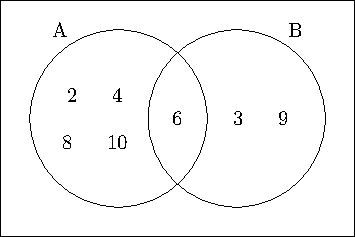
\includegraphics[width=0.35\linewidth]{tikz/VennEx2-1-6} 

}

\end{figure}

As previously discussed, sets do not have to just be composed of numbers. Moreover, sets can have many different relationships between them, as seen in Figure \ref{fig:venn-samples}. If a set is a subset of a second set, then they are visualized as one region inside of the other region. If there are elements shared between two sets, but are not known to have a subset relationship, then they are visualized as overlapping regions. If no elements of the two sets are the same, then they are represented as two non-overlapping regions. In the next section we define vocabulary to describe these different types of relationships and how they are combined in different ways.

\begin{figure}

{\centering 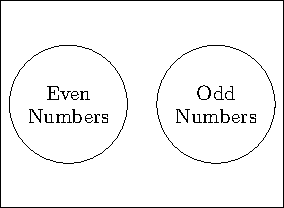
\includegraphics[width=0.3\linewidth]{tikz/evenodd} 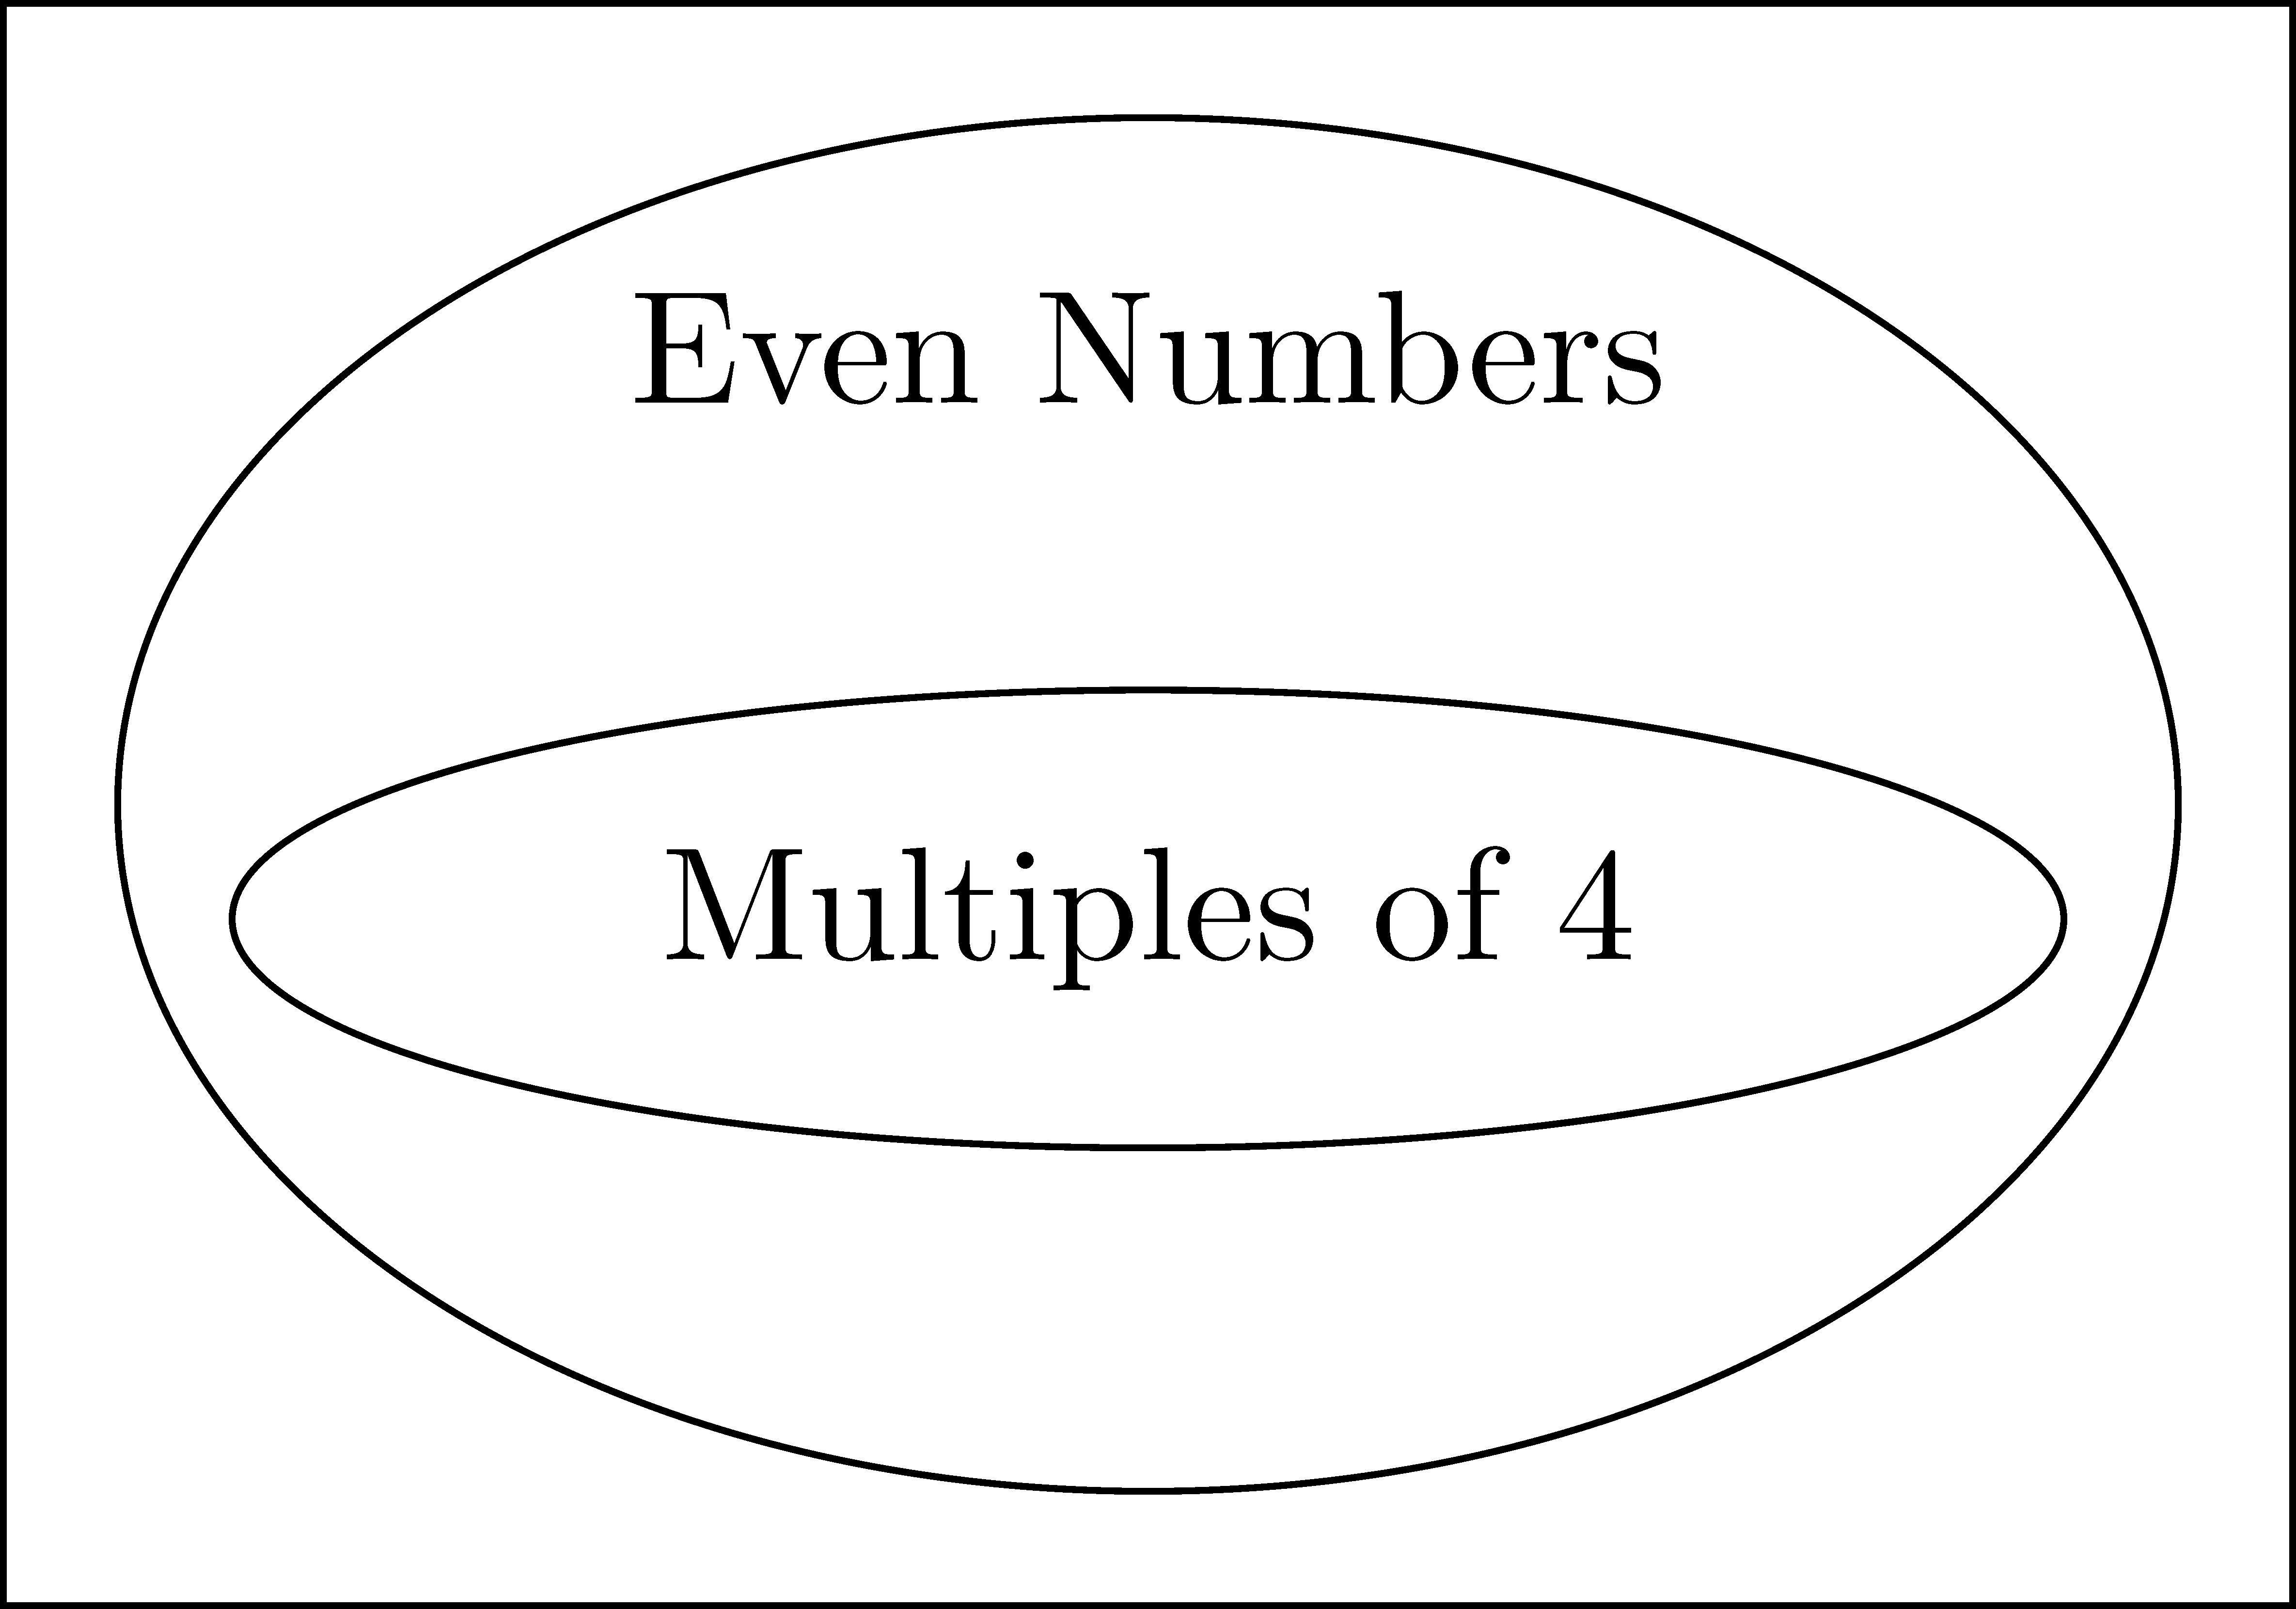
\includegraphics[width=0.3\linewidth]{tikz/evenfours} 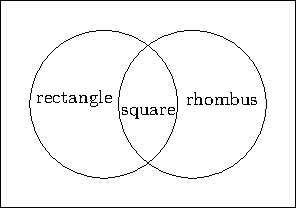
\includegraphics[width=0.3\linewidth]{tikz/rectsqrhombus} 

}

\caption{Sample Venn diagrams}\label{fig:venn-samples}
\end{figure}

\hypertarget{list-of-sets-of-numbers}{%
\subsection{List of Sets of Numbers}\label{list-of-sets-of-numbers}}

In order to help with terminology we will provide some notation for some of the basic sets used in the text.

We define the natural numbers as
\[\mathbb{N}=\{0,1,2,3,4,5,\ldots\}.\]
This is distinct from some definitions of the natural numbers that do not include the number \(0\). When a text defines the natural numbers without the \(0\), it also defines the whole numbers to be our definition of the natural numbers. We are including \(0\) due to the method in which we define the natural numbers in Chapter \ref{ch:number}.

We label the integers as \[\mathbb{Z} = \{\ldots, -4, -3, -2, -1, 0, 1, 2, 3, 4, \ldots\},\] which we will define in detail in Section \ref{sec:Integers}.

We label the set of rational numbers as \(\mathbb{Q}\) and the real numbers as \(\mathbb{R}\), the detailed definitions of which are in Sections \ref{sec:rationals} and \ref{sec:reals}, respectively.

The complex numbers, \(\mathbb{C}\), are defined and studied in Section \ref{sec:complex}.

For the integers, rationals and reals, we define \(\mathbb{Z}^+\), \(\mathbb{Q}^+\), and \(\mathbb{R}^+\) to be the positive elements of the set, those that are greater than zero.

We visualize the nested nature of these number systems in the Venn diagram in Figure \ref{fig:venn-numbers}.

\begin{figure}

{\centering 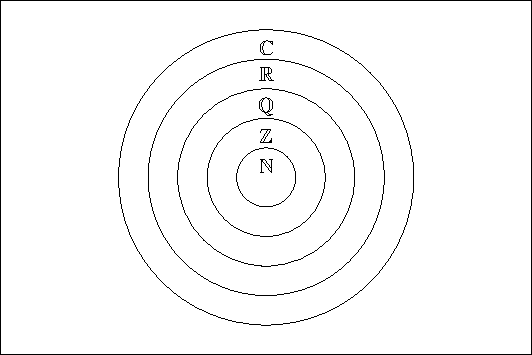
\includegraphics[width=0.7\linewidth]{tikz/vennNumberSystems} 

}

\caption{Sample Venn diagrams}\label{fig:venn-numbers}
\end{figure}

\hypertarget{exercises-3}{%
\subsection{Exercises}\label{exercises-3}}

\begin{enumerate}
\def\labelenumi{\arabic{enumi}.}
\item
  Answer the following as true or false. If false, explain why the statement is not true.

  \begin{enumerate}
  \def\labelenumii{\alph{enumii}.}
  \item
    \(\emptyset \subseteq \{f,u,n,t,i,m,e,s\}\)
  \item
    \(\{a,b\} \in \{a,b,c\}\)
  \item
    \(\{0 \}\ = \emptyset\)
  \item
    \(\{f,u,n,f,u,n \}=\{f,u,n \}\)
  \item
    \(\{0,0\} \subseteq \{0,0,1,1,2,2\}\)
  \end{enumerate}
\item
  Let \(A=\{1, 2, 3\}\), \(B=\{a, b, c\}\), and \(C=\{1, a, 2, b, 3, c\}\). Answer the following as true or false. If false, explain why the statement is not true.

  \begin{enumerate}
  \def\labelenumii{\alph{enumii})}
  \item
    \(A \subseteq A\)
  \item
    \(A\supseteq C\)
  \item
    \(A=B\)
  \item
    \(A \nsubseteq B\)
  \end{enumerate}
\item
  Recall that for set \(A\), \(\mathcal{P}(A)\) is the power set of \(A\).

  \begin{enumerate}
  \def\labelenumii{\alph{enumii})}
  \item
    Let \(A=\{a,b\}\). Write the set of \(\mathcal{P}(A)\) by listing its elements.
  \item
    Let \(A\) be a set with \(n\) elements in it.
  \item
    How many elements are in \(\mathcal{P}(A)\) if \(n=3\)?
  \item
    How many elements are in \(\mathcal{P}(A)\) if \(n=4\)?
  \item
    How many elements are in \(\mathcal{P}(A)\) if \(n\) is an unknown natural number?
  \end{enumerate}
\item
  Some textbooks describe a set as ``a well-defined collection of objects'' which means that the inclusion criteria that helps you decide what should be in the set is clearly specified. Classify each of the following sets as well-defined or not. If you identify a set as not well-defined, give two possible well-defined sets that would satisfy the original description.

  \begin{enumerate}
  \def\labelenumii{\alph{enumii})}
  \item
    \(\{x \vert x>0\}\)
  \item
    The set of students at The University of Awesome who are currently enrolled in a class that has a 100-level designation.
  \item
    \(\{x\vert x \textrm{ is a letter in my first name}\}\)
  \item
    The set of my friends.
  \item
    \(A_n=\{x\in \mathbb{Z} \vert n\leq x\leq n+3\}\)
  \end{enumerate}
\item
  Let \(A=\{1, 2, 3, 4\}\), \(B=\{7,8,9\}\), and \(C=\{3,4,5,6,7,8,9\}\). Using the most appropriate template of the Venn diagrams shown in Figure \ref{fig:venn-samples}, fill in the regions with the elements from:

  \begin{enumerate}
  \def\labelenumii{\alph{enumii})}
  \item
    Sets \(A\) and \(B\).
  \item
    Sets \(A\) and \(C\).
  \item
    Sets \(B\) and \(C\).
  \item
    Sets \(A\), \(B\), and \(C\) (you will have to make a new Venn diagram template).
  \end{enumerate}
\end{enumerate}

\hypertarget{algebra-of-sets}{%
\section{Algebra of Sets}\label{algebra-of-sets}}

Now that we understand the basic definitions involving sets, we examine set operations. These will allow us to create new sets from given sets.

\begin{definition}
\protect\hypertarget{def:unnamed-chunk-12}{}{\label{def:unnamed-chunk-12} }Let \(A\) and \(B\) be sets. We define the union of \(A\) and \(B\), denoted \(A \cup B\), to be the set of elements that are either in \(A\) or \(B\), or possibly both. We define the intersection of \(A\) and \(B\), \(A \cap B\), to be the set of elements that are in both \(A\) and \(B\). We say that \(A\) and \(B\) are \textbf{disjoint} if \(A\cap B = \emptyset\).
\end{definition}

The shaded regions in Figure \ref{fig:set-union} illustrate each set relationship in terms of general sets \(A\) and \(B\). We can also write the union and intersection of sets in terms of set-builder notation:
\[A\cup B = \{x \vert x\in A \mbox{ or } x\in B\} \quad \mbox{ and } \quad A\cap B =\{x\vert x\in A \mbox{ and } x\in B\}.\]

\begin{figure}

{\centering 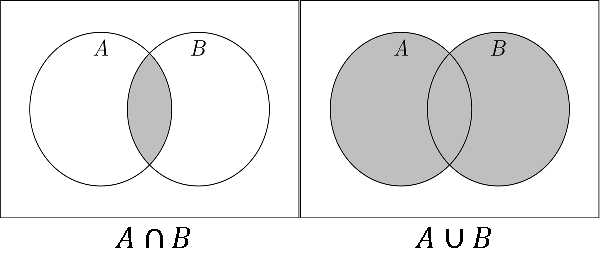
\includegraphics[width=0.7\linewidth]{tikz/Set_unions_intersections} 

}

\caption{The union and intersection of two sets}\label{fig:set-union}
\end{figure}

Let's look at a couple of examples to better understand these unions and intersections.

\begin{example}
\protect\hypertarget{exm:unnamed-chunk-13}{}{\label{exm:unnamed-chunk-13} } Let \(A = \{a, b, c, d, e\}\) and \(B = \{ d, e, f, g\}\). Then \[A\cup B=\{a, b, c, d, e, f, g\} \]
\end{example}

\begin{example}
\protect\hypertarget{exm:unnamed-chunk-14}{}{\label{exm:unnamed-chunk-14} } Let \(A=\{1,2,3,4,5,6,7,8,9\}\) and \(B=\{2,4,6,8\}\). Then
\[A \cup B = A \quad \mbox{ and } \quad A\cap B = B.\]
\end{example}

\begin{example}
\protect\hypertarget{exm:unnamed-chunk-15}{}{\label{exm:unnamed-chunk-15} } Let \(A=\{a,b,c\}\) and \(B=\{1,2,3\}\). Then
\[A\cup B = \{a,b,c,1,2,3\} \quad \mbox{ and } \quad A\cap B =\emptyset.\]
\end{example}

\begin{example}
\protect\hypertarget{exm:unnamed-chunk-16}{}{\label{exm:unnamed-chunk-16} } Let \(A = \{ x\in \mathbb{R} \: \vert \: x > 5\}\) and \(B=\{x \in \mathbb{R} \: \vert \: x < 8\}\). Then \(A\cup B\) would be all real numbers, since any real number is either less than 8 or greater than 5. And \(A\cap B\) would be the real numbers between 5 and 8. These can also be represented on number lines, where the shaded lines and filled dots are included in the set, with open dots and unshaded lines not being included in the set.
\end{example}

\begin{center}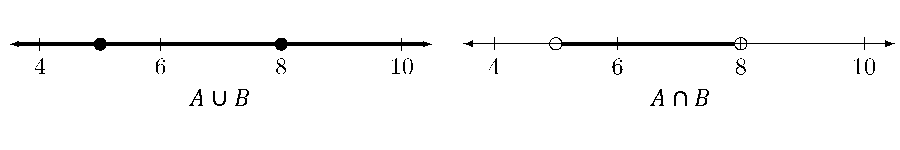
\includegraphics[width=0.95\linewidth]{tikz/number-line-unions} \end{center}

The following theorem identifies properties of the union as an operation on sets that follow from the definition.

\begin{theorem}
\protect\hypertarget{thm:unnamed-chunk-18}{}{\label{thm:unnamed-chunk-18} }Let \(A\), \(B\), and \(C\) be sets. Then we have the following:

\begin{enumerate}
\def\labelenumi{\arabic{enumi}.}
\item
  \(A\cup \emptyset = A\)
\item
  \(A \cup A = A\)
\item
  \(A \cup B = B \cup A\)
\item
  \(A \cup (B\cup C ) = (A\cup B) \cup C\)
\item
  \(A \subseteq A \cup B\)
\item
  If \(A \subseteq B\), then \(A\cup B=B\)
\end{enumerate}
\end{theorem}

\begin{proof}
\iffalse{} {Proof. } \fi{}The first two statements follow directly from the definition of the union. The empty set has no elements, making its union with \(A\) equal to \(A\). Because \(A\) and \(A\) have the same elements, the union must also be \(A\).

The third statement suggests that the set operation ``union'' is commutative, in that the order of the operation does not matter. The proof follows from properties of symbolic logic in relation to the use of the ``or'' statement in the definition of the union.

The fourth statement in the theorem is used to expand the definition of union, which is only defined for a pair of sets, to more than two sets. A further consequence of statement four is that the method of pairing sets the under the operation of union is irrelevant. We show this by proving the two statements \(A \cup (B\cup C ) \subseteq (A\cup B) \cup C\) and \((A\cup B) \cup C \subseteq A \cup (B\cup C)\) (see Theorem \ref{thm:set-equality}). In order to show the first containment, we let \(x\in A \cup (B\cup C )\) be a generic element. Then by the definition of the union of sets, \(x\in A\) or \(x\in (B\cup C)\). We will then break this statement into two cases.

\textbf{Case 1.} If \(x\in A\), then by the definition of unions \(x\in (A \cup B)\). Then using the definitions of unions again, \(x \in ((A \cup B) \cup C)\).

\textbf{Case 2.} If \(x\in (B\cup C)\), then \(x\in B\) or \(x\in C\). If \(x\in B\), then \(x\in (A\cup B)\) and also \(x\in ((A\cup B) \cup C)\). If \(x\in C\), then \(x\in ((A\cup B) \cup C)\).

So in either case, \(x \in A \cup (B\cup C)\) implies that \(x\in (A\cup B) \cup C\). So \(A\cup (B\cup C) \subseteq (A\cup B)\cup C\). The proof of the reverse containment is nearly identical.

We leave the last two statements as exercises.
\end{proof}

Similar to the union, the following theorem demonstrates how the intersection of sets works as an operation on sets. The proofs for each statement are similar to that of the unions so we will leave the proof of this theorem as an exercise.

\begin{theorem}
\protect\hypertarget{thm:intersections}{}{\label{thm:intersections} }Let \(A\), \(B\), and \(C\) be sets. Then we have the following

\begin{enumerate}
\def\labelenumi{\arabic{enumi}.}
\item
  \(A\cap \emptyset = \emptyset\)
\item
  \(A \cap A = A\)
\item
  \(A \cap B = B \cap A\)
\item
  \(A \cap (B\cap C ) = (A\cap B) \cap C\)
\item
  If \(A \subseteq B\), then \(A \cap B = A\)
\end{enumerate}
\end{theorem}

Now that we know how unions and intersections behave by themselves, we examine how they interact with each other.

\begin{theorem}
\protect\hypertarget{thm:set-distribution}{}{\label{thm:set-distribution} }Let \(A\), \(B\), and \(C\) be sets. Then
\[ A \cap (B \cup C) = (A \cap B) \cup (A \cap C) \quad \mbox{ and } \quad  A \cup (B \cap C) = (A \cup B) \cap (A \cup C).\]
\end{theorem}

These relationships are diagrammed in Figure \ref{fig:set-distributions}.

\begin{figure}

{\centering 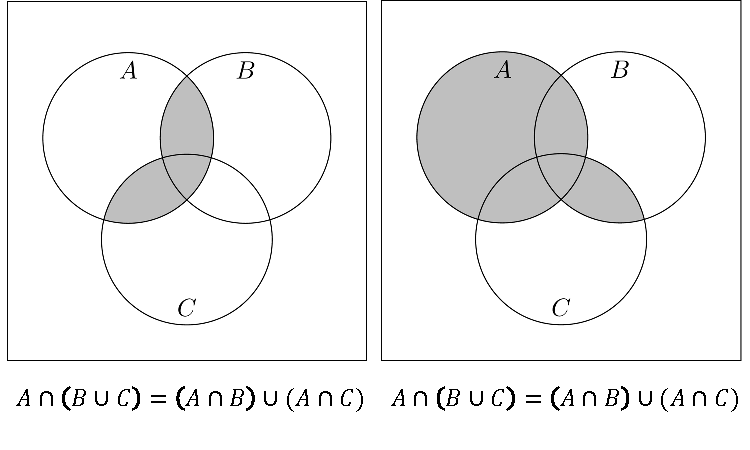
\includegraphics[width=0.8\linewidth]{tikz/set-distribution} 

}

\caption{Venn Diagrams for Set Distribuions }\label{fig:set-distributions}
\end{figure}

\begin{proof}
\iffalse{} {Proof. } \fi{} As each of these are proofs of equality of sets, we will need to complete the proofs showing that each set is contained in the other (see Theorem \ref{thm:set-equality}). We prove Part 1 and leave Part 2 as an exercise.

Let \(x\in A \cap (B \cup C)\). Then \(x\in A\) and \(x\in (B\cup C)\). This yields two cases: \(x\in A\) and \(x\in B\), or \(x\in A\) and \(x\in C\). This is equivalent to \(x \in (A\cap B) \cup (A\cap C)\). Thus \(A \cap (B \cup C) \subseteq (A \cap B) \cup (A \cap C)\).

If \(x\in (A \cap B) \cup (A \cap C)\), then we have to examine two cases: \(x\in (A\cap B)\) or \(x\in (A \cap C)\).

\textbf{Case 1.} If \(x\in (A\cap B)\), then \(x\in A\) and \(x\in B\). Since \(x\in B\), we know that \(x\in (B\cup C)\). Thus \(x\in A \cap (B\cup C)\).

\textbf{Case 2.} If \(x \in (A\cap C)\), then \(x\in A\) and \(x\in C\). Since \(x\in C\), we know that \(x \in (B\cup C)\). Thus \(x \in A \cap (B\cup C)\).

These results imply that \((A \cap B) \cup (A \cap C) \subseteq A \cap (B \cup C)\). Thus, the Part 1 of the theorem is proven.
\end{proof}

\hypertarget{set-complements}{%
\subsection{Set Complements}\label{set-complements}}

When working on a problem, we usually describe several sets, with an underlying assumption that the sets referenced contain elements from some common, larger set. We call a set that contains all of the elements considered for a particular situation a \textbf{universal set}.

\begin{definition}
\protect\hypertarget{def:unnamed-chunk-21}{}{\label{def:unnamed-chunk-21} }For every set \(A\) that is a subset of the universal set \(U\), we define the \textbf{complement} of \(A\) to be the set of elements in the universal set that are not in \(A\), denoted
\[A^c=\left\{ x\in U \middle \vert x \notin A\right\}.\]\\
\end{definition}

\begin{figure}

{\centering 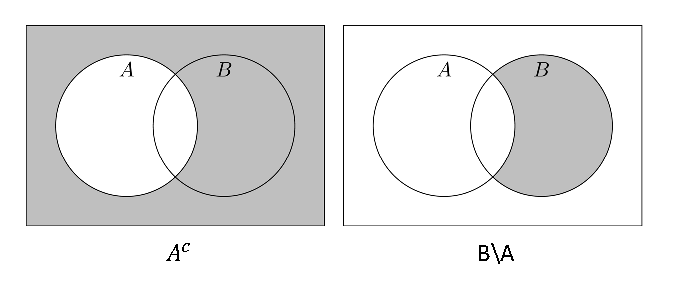
\includegraphics[width=0.8\linewidth]{tikz/set-difference} 

}

\caption{Set Complement and Set Difference}\label{fig:set-difference}
\end{figure}

For a given set \(A\) in universal set \(U\), the complement of a set identifies everything that is in the universal set except for things in set \(A\). This is often useful, however there are times when it is important to consider the elements that are in one set, but not in another, without reference to the universal set.

\begin{definition}
\protect\hypertarget{def:unnamed-chunk-22}{}{\label{def:unnamed-chunk-22} } Let \(A\) and \(B\) be sets. The complement of \(A\) with respect to \(B\), also called the \textbf{set difference} of \(B\) and \(A\), is defined as
\[B\setminus A = B \cap A^c = \left\{x\in B \middle \vert x \notin A\right\}.\]
\end{definition}

Let's revisit our previous examples to understand this idea of a set difference.

\begin{example}
\protect\hypertarget{exm:unnamed-chunk-23}{}{\label{exm:unnamed-chunk-23} } Let \(A = \{a, b, c, d, e\}\) and \(B = \{ d, e, f, g\}\). Then \[A\setminus B=\{a, b, c\} \quad \mbox{ and } \quad  B\setminus A =\{ f, g\}.\]
\end{example}

\begin{example}
\protect\hypertarget{exm:unnamed-chunk-24}{}{\label{exm:unnamed-chunk-24} } Let \(A=\{1,2,3,4,5,6,7,8,9\}\) and \(B=\{2,4,6,8\}\). Then
\[A \setminus B = \{1,3,5,7,9\} \quad \mbox{ and } \quad B\setminus A = \emptyset.\]
\end{example}

\begin{example}
\protect\hypertarget{exm:unnamed-chunk-25}{}{\label{exm:unnamed-chunk-25} } Let \(A=\{a,b,c\}\) and \(B=\{1,2,3\}\). Then
\[A\setminus B = A \quad \mbox{ and } \quad B\setminus A =B.\]
\end{example}

\hypertarget{de-morgans-laws}{%
\subsection{De Morgan's Laws}\label{de-morgans-laws}}

In the same year as the seminal work of Boole \citeyearpar{Boole} that started mathematics as a theoretical discipline, Augustus De Morgan published a foundational work in logic \citep{DeMorgan}. In this book, De Morgan defines and describes symbolic mathematical logic. His work has become the foundation for our current mathematical system. One of the key components of this work examines the complements of intersections and unions \citep[p.~69]{DeMorgan}.

\begin{theorem}[De Morgan's laws]
\protect\hypertarget{thm:unnamed-chunk-26}{}{\label{thm:unnamed-chunk-26} \iffalse (De Morgan's laws) \fi{} }If \(A\) and \(B\) are subsets of the same universal set, then
\[ \left(A \cap B\right)^c = A^c \cup B^c \quad \mbox{and} \quad \left(A \cup B \right)^c = A^c \cap B^c.\]
\end{theorem}

\begin{proof}
\iffalse{} {Proof. } \fi{} Because we are proving that two sets are equal we need to prove that the sets are subsets of each other. Here we will prove that \(\left(A \cap B\right)^c = A^c \cup B^c\) and leave the other proof as an exercise.

(Proof that \(\left(A \cap B\right)^c \subseteq A^c \cup B^c\).):

Let \(x\in \left(A \cap B\right)^c\). So \(x\) is not in \(A\cap B\). \(x\) is not in both \(A\) and \(B\).

Case 1. If \(x\in A\), then \(x\notin B\). So \(x\in B^c\).

Case 2. If \(x\notin A\), then \(x\in A^c\).

So either way, \(x\) is in \(A^c\) or \(x\) is in \(B^c\) (\(x\in A^c \cup B^c\)). Therefore, \(\left(A \cap B\right)^c \subseteq A^c \cup B^c\).

(Proof that \(A^c \cup B^c \subseteq \left(A \cap B\right)^c\).):

Let \(x \in A^c \cup B^c\).

Case 1. \(x\in A^c\). Then \(x\notin A\). So \(x\notin A\cap B\). So \(x\in (A\cap B)^c\).

Case 2. \(x\in B^c\). Then \(x\notin B\). So \(x\notin A\cap B\). So \(x\in A\cap B)^c\).

Therefore, \(A^c \cup B^c \subseteq \left(A \cap B\right)^c\)

Therefore, \(\left(A \cap B\right)^c = A^c \cup B^c\).
\end{proof}

It is also helpful to understand De Morgan's laws by looking at the corresponding Venn diagrams, shown in Figure \ref{fig:demorgan}.

\begin{figure}

{\centering 
\includegraphics[width=0.8\linewidth]{tikz/demorgan} 

}

\caption{Venn diagrams for De Morgan's laws for pairs of sets}\label{fig:demorgan}
\end{figure}

\hypertarget{subsec:cartesian}{%
\subsection{Cartesian Products}\label{subsec:cartesian}}

The previous sections have considered set operations between two sets that exist in the same universal set. Sets can also be combined to create new sets that exist in a universal set that differs from those of the sets used to create it. The collection of set operations that do this allows us to use sets to create multidimensional systems such as ordered pairs.

\begin{definition}
\protect\hypertarget{def:unnamed-chunk-28}{}{\label{def:unnamed-chunk-28} } The \textbf{Cartesian Product} of two non-empty sets \(A\) and \(B\) is the set
\[A\times B = \left\{ (a,b) \middle \vert a \in A, b\in B\right\}\] of all ordered pairs of elements where the first coordinate in the pair comes from the set \(A\) and the second coordinate is an element of \(B\).
\end{definition}

The most common Cartesian product in the secondary mathematics curriculum is real plane, \(\mathbb{R} \times \mathbb{R}\), which is often denoted by \[\mathbb{R}^2:= \left\{ (x,y) \vert x,y\in \mathbb{R} \right\}.\]

\begin{quote}
\hypertarget{related-content-standards-2}{%
\subsubsection*{Related Content Standards}\label{related-content-standards-2}}
\addcontentsline{toc}{subsubsection}{Related Content Standards}

\begin{itemize}
\tightlist
\item
  (5.G.1) Use a pair of perpendicular number lines, called axes, to define a coordinate system, with the intersection of the lines (the origin) arranged to coincide with the \(0\) on each line and a given point in the plane located by using an ordered pair of numbers, called its coordinates. Understand that the first number indicates how far to travel from the origin in the direction of one axis, and the second number indicates how far to travel in the direction of the second axis, with the convention that the names of the two axes and the coordinates correspond (e.g., \(x\)-axis and \(x\)-coordinate, \(y\)-axis and \(y\)-coordinate).
\end{itemize}
\end{quote}

The concept of the Cartesian product can be generalized to more than a pair of sets, for example \[\mathbb{R}^3:= \left\{ (x,y,z) \vert x,y,z\in \mathbb{R} \right\}\] is the three dimensional Cartesian space where each coordinate is a real number.

\begin{theorem}
\protect\hypertarget{thm:set-identities}{}{\label{thm:set-identities} }It is sometimes helpful to summarize all of the properties of algebra on sets into a single location.

Let all sets referred to below be subsets of a universal set \(U\).

\begin{enumerate}
\def\labelenumi{\arabic{enumi}.}
\item
  (Commutative Laws) For all sets \(A\) and \(B\),
  \[(a) \: A \cup B = B \cup A \quad \mbox{and} \quad (b) \: A \cap B = B \cap A\]
\item
  (Associative Laws) For all sets \(A\), \(B\), and \(C\),
  \[(a) \: (A\cup B)\cup C = A \cup (B \cup C) \quad \mbox{and} \quad (b) \: (A \cap B) \cap C = A \cap (B\cap C)\]
\item
  (Distributive Laws) For all sets \(A\), \(B\), and \(C\),
  \[(a) \: A \cup (B \cap C) = (A \cup B)\cap (A \cup C) \quad \mbox{and} \quad (b) \: A \cap (B \cup C) = (A \cap B)\cup (A \cap C)\]
\item
  (Identity Laws) For all sets \(A\),
  \[(a) \: A \cup \emptyset = A \quad \mbox{and} \quad (b) \: A \cap U = A\]
\item
  (Complement Laws)
  \[(a) \: A \cup A^c = U \quad \mbox{and} \quad (b) \: A \cap A^c = \emptyset\]
\item
  (Double Complement Law) For all sets \(A\),
  \[(A^c)^c =A\]
\item
  (Idempotent Laws) For all sets \(A\),
  \[(a) \: A\cup A=A \quad \mbox{and} \quad (b) \: A \cap A =A\]
\item
  (Universal Bound Laws) For all sets \(A\),
  \[(a) \: A \cup U = U\quad \mbox{and} \quad (b) \: A \cap \emptyset = \emptyset\]
\item
  (De Morgan's Laws) For all sets \(A\) and \(B\),
  \[(a) \: (A \cup B)^c = A^c \cap B^c\quad \mbox{and} \quad (b) \: (A \cap B)^c = A^c \cup B^c\]
\item
  (Absorption Laws) For all sets \(A\) and \(B\),
  \[(a) \: A \cup (A \cap B) = A \quad \mbox{and} \quad (b) \: A \cap (A \cup B ) = A\]
\item
  (Complements of \(U\) and \(\emptyset\))
  \[(a) \: U^c = \emptyset \quad \mbox{and} \quad (b) \: \emptyset^c = U\]
\item
  (Set Difference Law) For all sets \(A\) and \(B\),
  \[A\setminus B = A \cap B^c\]
\end{enumerate}
\end{theorem}

\hypertarget{exercises-4}{%
\subsection{Exercises}\label{exercises-4}}

\begin{enumerate}
\def\labelenumi{\arabic{enumi}.}
\item
  Middle and high school students often struggle to remember the difference between union and intersection.

  \begin{enumerate}
  \def\labelenumii{\alph{enumii})}
  \tightlist
  \item
    Describe a memory trick to help students remember which symbol goes with which of the two operations.
  \item
    Review the definitions of the intersection and union of two sets. What key words separate the two definitions from each other?
  \item
    Some students, when first learning the mathematical definition of union, think that the definition excludes objects that are in both sets. These students, when given two sets and asked to find \(A \cup B\) will include the items that are in \(A\) only and \(B\) only. They exclude things in \(A \cap B\). What might be the source of this misconception?
  \item
    Define a non-numeric universe and two sets, \(A\) and \(B\), in your universe such that \(A \cap B \neq \emptyset\). Describe, using words, each of the following sets:

    \begin{enumerate}
    \def\labelenumiii{\roman{enumiii}.}
    \tightlist
    \item
      \(A \cup B\)
    \item
      \(A \cap B\)
    \item
      \(A^{C}\)
    \end{enumerate}
  \end{enumerate}
\item
  Let \(A = \{1, 3, 5, 7, 9\}\), \(B=\{1, 2, 3, 4\}\), and \(C=\{3, 6, 9\}\). List the elements of each of the specified sets.

  \begin{enumerate}
  \def\labelenumii{\alph{enumii}.}
  \tightlist
  \item
    \(A \cap B\)
  \item
    \(A \cup B\)
  \item
    \(A \cup C\)
  \item
    \((A\cap B) \cup C\)
  \item
    \(A \cap (B \cup C)\)
  \item
    \(A \times B\)
  \item
    \(B \times (A\cap C)\)
  \end{enumerate}
\item
  For this exercise, assume that \(\mathbb{R}\) is the universal set. For any natural number, \(n\), define \(n\mathbb{Z} = \{nx \vert x \in \mathbb{Z}\}\). Answer the following as true or false. If false, explain why the statement is not true.

  \begin{enumerate}
  \def\labelenumii{\alph{enumii}.}
  \tightlist
  \item
    \((2\mathbb{Z})^C = \{2x+1 \vert x \in \mathbb{Z}\}\)
  \item
    \(\mathbb{R}\setminus \mathbb{Z}=\mathbb{Z}^C\)
  \item
    \(5\mathbb{Z} \cap \{2x+1 \vert x \in \mathbb{Z}\} = 5\mathbb{Z}\)
  \item
    \(5\mathbb{Z} \cap 4\mathbb{Z} = 20\mathbb{Z}\)
  \item
    \(2\mathbb{Z}\setminus (4\mathbb{Z} \cup 6\mathbb{Z})= \emptyset\)
  \item
    \(3\mathbb{Z}\setminus 2\mathbb{Z}=\{3(2x-1) \vert x\in \mathbb{Z} \textrm{ and } x\geq 0\}\)
  \end{enumerate}
\item
  Let \(A\) and \(B\) be sets. Prove that \(A\subseteq A\cup B\).
\item
  Let \(A\) and \(B\) be sets. Prove that if \(A\subseteq B\), then \(A\cup B=B\).
\item
  Prove Theorem \ref{thm:intersections}.
\item
  Prove Part 2 of Theorem \ref{thm:set-distribution}.
\item
  Prove that for sets \(A\) and \(B\), \((A\cap B)^c = A^c \cup B^c\) and \((A\cup B)^c=A^c\cap B^c\)
\item
  Write \((A\setminus B)\cup (B\setminus A)\) in terms of just unions, intersections, and complements, then simplify your expression.
\item
  Often when doing mathematics, the set you are working with or within is left unstated.

  \begin{enumerate}
  \def\labelenumii{\alph{enumii}.}
  \tightlist
  \item
    Under what conditions is it important to be explicit with students about the set you are working within?
  \item
    What set do you assume you are working in when:

    \begin{enumerate}
    \def\labelenumiii{\arabic{enumiii}.}
    \tightlist
    \item
      You are figuring out how much something will cost?
    \item
      You are figuring out what proportion of a pizza to give everyone?
    \item
      You are determining what the temperature will be if it is predicted to drop 20 degrees overnight?
    \end{enumerate}
  \end{enumerate}
\item
  Construct an algebraic proof for the given statement. Cite a property from Theorem \ref{thm:set-identities} for every step.
\end{enumerate}

\begin{quote}
For all sets \(A\) and \(B\), \[A \cup (B-A)= A \cup B\]
\end{quote}

\hypertarget{collections-of-sets}{%
\section{Collections of Sets}\label{collections-of-sets}}

Now that we know how to combine pairs of sets, we can inductively define unions and intersections for a finite or infinite number of sets.

When we are dealing with more than one or two related but distinct sets we often use another set as an \textbf{index set} in order to more easily describe and distinguish the sets in the collection.

\begin{example}
\protect\hypertarget{exm:unnamed-chunk-29}{}{\label{exm:unnamed-chunk-29} }Let the natural numbers, \(\mathbb{N}=\{1, 2, 3, \ldots \}\), be an indexing set. For each natural number, \(n\), we define \[A_n = [n,n+1),\] which is an interval in the real numbers. In this situation, we have
\[A_1 = [1,2), \:  A_2 = [2,3), \: A_3 = [3,4),\:  \ldots \]
In this case, the use of \(\mathbb{N}\) tells us that we have an infinite set of sets. We use the indexing set to express the form of a general interval. When we assign an index value (such as \(n=3\)), we are effectively identifying a particular interval in the sequence of intervals.
\end{example}

Using indexing sets, we can then define the union and intersection of a collection of sets.

\begin{definition}
\protect\hypertarget{def:unnamed-chunk-30}{}{\label{def:unnamed-chunk-30} } Let \(S\) be an indexing set and let \(\left\{ A_i\right\}_{i\in S}\) be an indexed non-empty family of sets. Then we define the union and intersection of the family of sets as
\[\bigcup_{i\in S} A_i = \left\{ x \middle \vert x\in A_i \mbox{ for some } i\in S\right\} \quad \mbox{ and } \quad \bigcap_{i\in S} A_i = \left\{ x\middle \vert x\in A_i \mbox{ for all } i \in S\right\}.\]
\end{definition}

\begin{example}
\protect\hypertarget{exm:disjoint}{}{\label{exm:disjoint} }Continuing with our previous example where \(A_n= [n,n+1)\) for each \(n\in \mathbb{N}\), we can write
\[ \bigcup_{i\in \{1,2,3\}} A_i = [1,4) \quad \mbox{and} \quad \bigcap_{i\in \{1,2,3\}} A_i = \emptyset\]
since the sets \(A_1\), \(A_2\), \(A_3\), and \(A_4\) do not overlap. If we extend this to the entire indexing set, then \[\bigcup_{i\in \mathbb{N}} A_i = [1,\infty) \quad \mbox{and} \quad \bigcap_{i\in \mathbb{N}} A_i = \emptyset.\]
\end{example}

An indexed collection of sets \(\{A_i\}_{i\in S}\) is called \textbf{mutually disjoint} if, for any \(i,j\in S\) with \(i\neq j\), \(A_i \cap A_j = \emptyset\). The sets in the previous example are mutually disjoint since \([n,n+1) \cap [m,m+1) = \emptyset\) if \(m\neq n\).

\begin{example}
\protect\hypertarget{exm:unnamed-chunk-31}{}{\label{exm:unnamed-chunk-31} }For each positive integer \(n\), (\(n\in \mathbb{N}\)), let \[S_n= \left\{x\in \mathbb{R}\middle \vert \frac{-1}{n} < x < \frac{1}{n} \right\}.\]

\[S_1=(-1,1)\]
\end{example}
\begin{figure}

{\centering 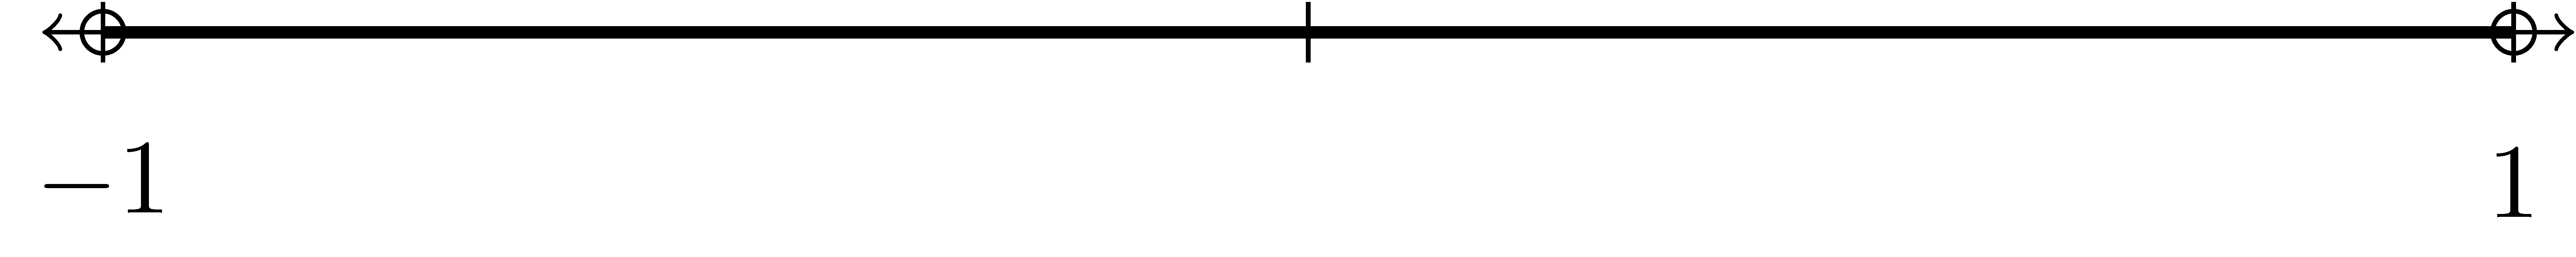
\includegraphics[width=0.35\linewidth]{tikz/Nested_s1} 

}

\end{figure}

\[S_2=(\frac{-1}{2}, \frac{1}{2})\]

\begin{figure}

{\centering 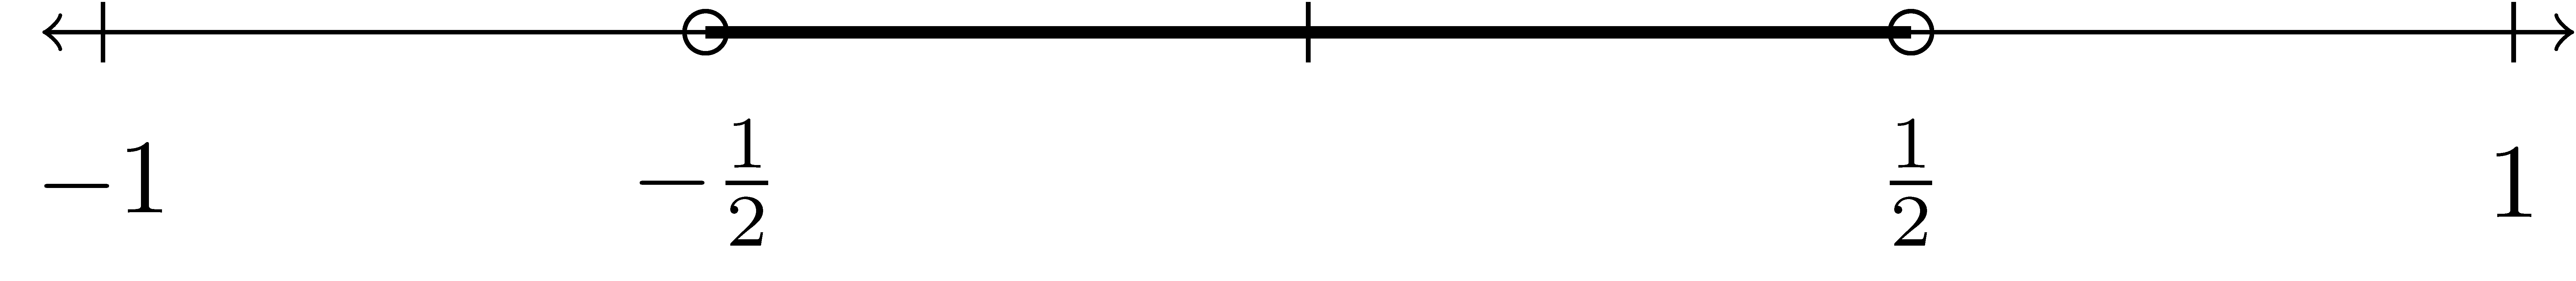
\includegraphics[width=0.35\linewidth]{tikz/Nested_s2} 

}

\end{figure}

\[S_3=(\frac{-1}{3}, \frac{1}{3})\]

\begin{figure}

{\centering 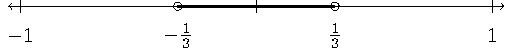
\includegraphics[width=0.35\linewidth]{tikz/Nested_s3} 

}

\end{figure}

Then we can see that for any \(i<j\), we have that \(S_i\cap S_j = S_j\) and \(S_i \cup S_j = S_i\).

We can also take the union and intersections over the entire collection of sets.
\[ \bigcup_{n\in \mathbb{N}} S_n = (-1,1) \quad \mbox{ and } \quad \bigcap_{n\in \mathbb{N}} S_n = \{0\}.\]

The above example is also an example of what is called a \textbf{nested} collection of sets.

\begin{definition}
\protect\hypertarget{def:unnamed-chunk-35}{}{\label{def:unnamed-chunk-35} } An indexed collection of sets, \(\left\{ A_i\right\}_{i\in I}\), with an order on \(I\) is called \textbf{nested} if either
\[ A_i \subseteq A_j \mbox{ whenever } i<j \quad \mbox{or} \quad A_i \supseteq A_j \mbox{ whenever } i<j.\]
When the indexing set is the natural numbers this is often denoted by \[A_0 \subseteq A_1 \subseteq A_2 \subseteq \cdots \quad \mbox{ or } \quad A_0 \supseteq A_1 \supseteq A_2 \supseteq \cdots.\]
\end{definition}

Using the ideas of indexing sets and families of sets, we can generalize De Morgan's Laws to a general collection of sets, the proofs of which are very similar to the proof in the case of two sets.

\begin{theorem}[Generalized De Morgan's Laws]
\protect\hypertarget{thm:unnamed-chunk-36}{}{\label{thm:unnamed-chunk-36} \iffalse (Generalized De Morgan's Laws) \fi{} }Let \(I\) be an indexing set and let \(\{A_i\}_{i\in I}\) be a collection of sets that are all subsets of the same universal set. Then
\[\left( \bigcup_{i\in I} A_i \right)^c = \bigcap_{i \in I} A_i^c \quad \mbox{and} \quad \left( \bigcap_{i\in I} A_i \right)^c = \bigcup_{i \in I} A_i^c\]
\end{theorem}

\hypertarget{exercises-5}{%
\subsection{Exercises}\label{exercises-5}}

\begin{enumerate}
\def\labelenumi{\arabic{enumi}.}
\item
  For each of the following collections of sets:

  \[\displaystyle{\mathcal{A} = \left\{ \left[ \frac{1}{n},n\right) \right\}_{n=2,3,4,\ldots }}\]

  \[\displaystyle{\mathcal{B} = \left\{ \left( n,\infty \right) \right\}_{n=0,1,2,3,4,5,\ldots} }\]

  \[\displaystyle{\mathcal{C} = \left\{ \left[ -n, n \right] \right\}_{n=0,1,2,3,4,5,\ldots }}\]

  \[\displaystyle{\mathcal{D} = \left\{ [x,x+1)\right\}_{x\in \mathbb{R}}}\]

  \[\displaystyle{\mathcal{E} = \left\{ \{z\in \mathbb{C}\middle \vert|z|=r\}\right\}_{r\in \mathbb{R}^+} }\]

  \[\displaystyle{\mathcal{F} = \left\{ \{n\in \mathbb{Z}\middle \vert n=3k+j \mbox{ for some } k\in \mathbb{Z}\}\right\}_{j=0,1,2}}\]

  \begin{enumerate}
  \def\labelenumii{\alph{enumii}.}
  \tightlist
  \item
    Determine if the sets are mutually disjoint
  \item
    Determine if the collection is nested
  \item
    Find the union of the collection
  \end{enumerate}
\end{enumerate}

\hypertarget{ch:equivalence}{%
\chapter{Equality, Order, and Equivalence}\label{ch:equivalence}}

The chapter title may look like just a list, but the notions of equality, order, and equivalence are a critically important trio of related but distinct ideas in mathematics. Together they help us define when two things are the ``same.'' Instruction in these ideas starts on almost the first day of school when students first learn how to count. Students continue study and expand these ideas in their study of mathematics: many of the theorems of mathematics labeled as ``Fundamental'' are statements of equivalence. These include the Fundamental Theorem of Arithmetic that every integer can be uniquely factored into primes, the Fundamental Theorem of Calculus describing the relationship between antiderivatives and infinite sums, and isomorphism theorems of abstract algebra and homeomorphisms of topology.

\hypertarget{partitions-and-equivalence-relations}{%
\section{Partitions and Equivalence Relations}\label{partitions-and-equivalence-relations}}

\begin{figure}

{\centering 
\includegraphics[width=0.5\linewidth]{images/m-and-m-1308543_1920} 

}

\caption{Sorting Candy}\label{fig:unnamed-chunk-37}
\end{figure}

As a way to better understand the world, humans tend to sort information into categories or orderings. For instance, when some people see a pile of various types of M\&M'sTM they have the urge to sort them in various ways. Some people sort the candies according to their color. Others may sort them according to their type (plain, peanut, etc.). This process of sorting is a type of ``partitioning'' the items into distinct categories. With this categorization we want to make sure that each candy is sorted into one, and only one, type. This type of sorting can be formalized with the following definition.

\hypertarget{partitions}{%
\subsection{Partitions}\label{partitions}}

\begin{definition}
\protect\hypertarget{def:unnamed-chunk-38}{}{\label{def:unnamed-chunk-38} } A \textbf{partition} of a set \(A\) is a finite or infinite collection of non-empty, mutually-disjoint subsets whose union is \(A\). \index{Partition}
\end{definition}

\begin{figure}

{\centering 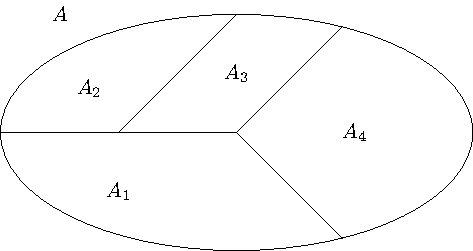
\includegraphics[width=0.5\linewidth]{tikz/Set_partition} 

}

\caption{Partition of Sets}\label{fig:unnamed-chunk-39}
\end{figure}

Thus, a partition of a set is a collection of subsets of the original set with several key properties. First, the subsets are non-empty, meaning that each subset in the partition contains at least one element. This allows us to restrict the partition to a collection of non-trivial subsets and means partitions have a type of uniqueness. The subsets in the partition are also mutually-disjoint which means that no element of the original set is in more than one of the subsets in the partition. Lastly, since the union of the subsets that form the partition is \(A\), we have that every element in \(A\) is in one of these subsets. Thus, each component of the definition of a partition is essential to defining a way to split a set into a set of categories that we find useful.

\begin{example}
\protect\hypertarget{exm:unnamed-chunk-40}{}{\label{exm:unnamed-chunk-40} }If we have a set
\[A=\left\{ a, 2, \alpha , \mbox{apple} , \mbox{box}, \beta, 1, 3, \gamma , \mbox{cow}, c, b \right\}\] there are some natural ways to partition the set. Here are three possible partitions.

\[
            A_1 = \{a,b,c\}, \:
            A_2 = \{1,2,3\},\: 
            A_3 = \{\alpha, \beta, \gamma\}, \: 
            A_4 = \{\mbox{apple} , \mbox{box}, \mbox{cow}\} 
\]
\[
            A_1 = \{\mbox{apple} , \mbox{box}, \mbox{cow}\}, \:
            A_2 = \{a,b,c,1,2,3,\alpha,\beta,\gamma\}
\]
\[
            A_1 = \{a,1,\alpha,\mbox{apple}\}, \: 
            A_2 = \{b,2,\beta,\mbox{box}\}, \: 
            A_3 = \{c,3,\gamma, \mbox{cow} \}
\]

There are many other ways to partition the set, but we do not have the space to write out all of the possible partitions of this set.
\end{example}

\begin{example}
\protect\hypertarget{exm:unnamed-chunk-41}{}{\label{exm:unnamed-chunk-41} } Early in the K-12 mathematics curriculum we ask students to determine which integers are even and which are odd. In this situation, the set \(A\) is the set of integers (\(\mathbb{Z}\)), while the subsets that form the partition are the subset of even numbers, (\(2\mathbb{Z}\)), and odd numbers, (\(2\mathbb{Z}+1\)).
\end{example}

\begin{example}
\protect\hypertarget{exm:unnamed-chunk-42}{}{\label{exm:unnamed-chunk-42} }If we let the set \(B\) be defined by the following list of elements,
\[B = \begin{Bmatrix} 
\mbox{ jar},  & \mbox{ jellybean} ,  & \mbox{ applesauce}, & \mbox{ ape}, & \mbox{ bear}, \\
\mbox{ ball}, & \mbox{ beanbag}, & \mbox{ bag}, & \mbox{ arm} , & \mbox{ skate} , \\
\mbox{ bike}, & \mbox{ rock}, & \mbox{ rowboat},   &  \mbox{ jigsaw}, & \mbox{ saw}
 \end{Bmatrix}\]
take some time to create various partitions of the set \(B\), verifying the various properties in the definition of a partition.
\end{example}

In this text, we denote the partition \(\mathcal{P}\) of a set \(A\) as the union of subsets of \(A\) over some indexing set, \(I\). For example, if the partition is formed using two subsets of \(A\), then the indexing set could be \(I=\{1,2\}\). The indexing set can also be infinite. For instance,
\[\mathcal{P} = \left\{ A_n  \right\}_{n\in \mathbb{Z}}, \: \mbox{ where } A_n=\left\{x\in \mathbb{R}\middle \vert n\leq x < n+1  \right\}\] is a partition of the real numbers with an infinite number of sets.

It is important to note that there are usually many ways to partition a set, but the definition of partition does not impose any constraints on the uniformity or order of the subsets, only that the way we choose our subsets meets the three conditions described previously.

With our previous discussion and examples in mind, we can translate our verbal definition of a partition into a symbolic one. In particular: if \(\mathcal{P}= \left\{ U_i\right\}_{i\in I}\) is a partition of a set \(A\), where \(I\) is some indexing set that is either finite or infinite, we have the following properties
\[U_i \bigcap U_j = \emptyset \quad \mbox{if } i\neq j, \quad \bigcup_{i\in I} U_i = A \mbox{, and} \quad U_i \neq \emptyset \mbox{ for all } i \in I.\]

\hypertarget{relations}{%
\subsection{Relations}\label{relations}}

Up until this point we have focused on building a framework for understanding the notion of partition. In order to understand the main topics of this chapter, we also need to develop the idea of a relation. While we give the general definition of a relation and a few examples, we will focus on those relations that arise from partitions in this section. We will explore other types of relations in later sections.

\begin{definition}
\protect\hypertarget{def:unnamed-chunk-43}{}{\label{def:unnamed-chunk-43} }Let \(A\) and \(B\) be sets. We define a relation \(R\) from \(A\) to \(B\) as a subset of \(A\times B\). We say that for elements \(a\in A\) and \(b\in B\) that \(a\) is related to \(b\), (\(aRb\)), if and only if \((a,b)\in R\). If the two sets are the same set, \(A\), then we say that \(R\) is a relation on \(A\).
\end{definition}

Here are some examples of relations in the K-12 curriculum.

\begin{itemize}
\item
  Let \(A\) and \(B\) be the set of integers. We could say that \[R=\{(a,b)\in A\times B \vert a<b\},\] which defines the `less than' relation of \(aRb \leftrightarrow a<b\).
\item
  Let \(A\) be the real numbers and \(B\) be the non-negative real numbers. We can let \[R=\{(x,y)\in A\times B \vert y=x^2\}.\] This is the graph of the function \(f(x)=x^2\).
\item
  Let \(A\) and \(B\) be the set of integers. We can define \[R= \{(m,n) \vert m-n=2k, \: \mbox{ for some integer } k\}.\] This relation is one where are the even numbers are related to each other and all of the odd numbers are related to each other.
\end{itemize}

\hypertarget{equivalence-relations-induced-by-partitions}{%
\subsection{Equivalence Relations Induced by Partitions}\label{equivalence-relations-induced-by-partitions}}

For the remainder of this section we will study a specific type of relation that is created by a partition, \(\mathcal{P}\), of a set, \(A\). If \(\mathcal{P}=\left\{U_i\right\}_{i\in I}\) is a partition of \(A\), we can write \(A\) as the union of a collection of non-empty, mutually disjoint subsets: \[U_i \cap U_j = \emptyset \mbox{ if } i\neq j, \: \mbox{ for each } i \in I, \: U_i\neq \emptyset, \: \mbox{ and } A=\bigcup_{i\in I} U_i.\]

Consider one of the individual subsets in the partition, say \(U_i\). Then the elements of \(U_i\), by virtue of the fact they are in the same subset, have a relationship to each other. This idea extends to the whole partition. That is, the partition induces a relation on \(A\) in the following way. For each \(a,b\in A\) we say that \(aRb\) if, and only if, there is a set \(U_i\) in the partition \(P\) such that both \(a\) and \(b\) are in \(U_i\).

The relations we create through a partition behave in ways that are of general interest in the study of mathematics.

If we choose a generic element \(a\) in \(A\), the property that \(\bigcup_{i\in I} U_i = A\) tells us that there exists \(i\in I\) such that \(a \in U_i\). So for every element \(a\in A\), we have that \(aRa\). We will call this property of the relation the \textbf{reflexive property}.

For the second property, if we have \(a,b\in A\) such that \(aRb\), then there must be a \(U_i\in P\) with \(a,b\in U_i\). This also means that \(bRa\). When you have the property that \(aRb\) implies that \(bRa\), we say that the relation has the \textbf{symmetric property}.

The third property of relations that we define derives from the property of partitions that
\[U_i \bigcap U_j = \emptyset \Leftrightarrow i\neq j.\] If \(a,b,c\in A\) such that \(aRb\) and \(bRc\), then we have that there are sets \(U_i\) and \(U_j\) in the partition such that \(a\) and \(b\) are both in \(U_i\) and \(b\) and \(c\) are both in \(U_j\). Since \(b\) is in both \(U_i\) and \(U_j\), \(U_i \cap U_j \neq \emptyset\) and so \(i=j\). This would then imply that \(aRc\). This property that the combination of \(aRb\) and \(bRc\) implies that \(aRc\) is called the \textbf{transitive property} of relations.

Not all relations have these three properties of reflexive, symmetric, and transitive. Those relations that have all three properties are called \textbf{equivalence relations}.

We have therefore proven that a partition of a set induces an equivalence relation on that set.

\hypertarget{partitions-induced-by-equivalence-relations}{%
\subsection{Partitions Induced by Equivalence Relations}\label{partitions-induced-by-equivalence-relations}}

The concept of equivalence relation is one that transcends much of mathematics and we often consider things as being the ``same'' with respect to some property if there is an equivalence relation under which they are related. One location that this appears in the elementary school curriculum is in regards to rational numbers. We think of \(\frac{1}{2}\) and \(\frac{2}{4}\) as being the same rational number, but written in a different way. Along these lines we say that two rational expressions \(\frac{a}{b}\) and \(\frac{c}{d}\) are equivalent if and only if \(ad=bc\). This creates and equivalence relation between these rational expressions that are used to create the rational numbers.

Similarly, if a relation, \(R\), on a set, \(A\), is an equivalence relation, then one can generate an induced partition, \(\mathcal{P}\), as follows. For each \(a\in A\) we define the set \[[a]_R := \left\{ b\in A \middle \vert aRb\right\}.\] We call this set, \([a]_R\), the equivalency class of \(a\) under the relation \(R\).

Since \(R\) is an equivalence relation, it is reflexive and so \(a \in [a]_R\) causing \([a]_R \neq \emptyset\). Since \(a\in [a]_R\), we have that \[\bigcup_{a\in A} [a]_R = A.\] Thus to show that \(\mathcal{P} = \left\{ [a]_R \middle \vert a \in A\right\}\) is a partition of \(A\), we need to show that for \(a,b\in A\) that \([a]_R=[b]_R\) or \([a]_R\bigcap [b]_R = \emptyset\).

If \([a]_R \bigcap [b]_R \neq \emptyset\), then we need to prove that two sets to be equal.

Let us assume that there exists a \(c\in [a]_R \bigcap [b]_R\).

Let \(d\in [a]_R\). So \(a R d\). \(c\) is also in \([a]_R\) and so \(aRc\). Since \(R\) is symmetric and \(aRd\), \(dRa\). We now have that \(dR c\) using transitive property. \(c\) is also in \([b]_R\) and so \(bRc\). Using the symmetric property, we have \(cR b\). Combining this with \(dRc\) and using the transitive property we have \(dR b\). Using the symmetric property we have \(bR d\). So \(d\in [b]_R\). Therefore, \([a]_R \subseteq [b]_R\).

Using very similar arguments we can prove that \([b]_R \subseteq [a]_R\).

So if the intersection is nonempty, the two sets are the same set.

We have thus proven the following theorem showing the connection between equivalence classes and partitions.

\begin{theorem}
\protect\hypertarget{thm:unnamed-chunk-44}{}{\label{thm:unnamed-chunk-44} }If \(R\) is an equivalence relation on a set \(A\), then \[P = \left\{ [a]_R \middle \vert a \in A\right\}\] is a partition of \(A\).

Similarly, if \(P= \left\{ U_i \middle \vert i \in I\right\}\) is a partition on a set \(A\), then the relation \(R\) defined by
\[aRb \Leftrightarrow \mbox{ there exists } i \in I \mbox{ such that } a,b \in U_i\] is an equivalence relation.
\end{theorem}

\hypertarget{exercises-6}{%
\subsection{Exercises}\label{exercises-6}}

\begin{enumerate}
\def\labelenumi{\arabic{enumi}.}
\item
  Define a relation \(\sim\) on \(\mathbb{R}\times (\mathbb{R}-\{0\})\) by
  \[(x,y) \sim (z,w) \Leftrightarrow xw=yz.\]

  \begin{enumerate}
  \def\labelenumii{\alph{enumii}.}
  \tightlist
  \item
    Show that this relation is an equivalence relation.
  \item
    Give a description of the partition of \(\mathbb{R}\times (\mathbb{R}-\{0\})\) induced by this equivalence relation.
  \item
    Why do we not allow \(0\) in the second part of the ordered pairs?
  \end{enumerate}
\item
  Determine which of the following collections of sets form a partition of \(\mathbb{R}\times \mathbb{R}\). For those that do form a partition, define the equivalence relation.

  \begin{enumerate}
  \def\labelenumii{\alph{enumii}.}
  \tightlist
  \item
    For \(c\in \mathbb{R}\), let \(h_c= \{ (x,y)\in \mathbb{R}^2 \vert y=c\}\), and let \(\mathcal{C} = \{h_c\}_{c\in \mathbb{R}}\).
  \item
    For \(m\in \mathbb{R}\), let \(s_m=\{ (x,y)\in \mathbb{R}^2 \vert y=mx\}\), and let \(\mathcal{D}= \{s_m\}_{m\in \mathbb{R}}\).
  \item
    For \(r\in [0,\infty)\), let \(C_r=\{ (x,y) \in \mathbb{R}^2 \vert x^2+y^2=r^2\}\), and let \(\mathcal{E}=\{C_r\}_{r\in [0,\infty)}\).
  \end{enumerate}
\item
  (For students who have knowledge of linear algebra) Let \(M_{2,2}\) be the set of \(2 \times 2\) matrices with real coefficients. For each of the following, prove that it is an equivalence relation, or show that one of the properties of equivalence relations does not hold.

  \begin{enumerate}
  \def\labelenumii{\alph{enumii}.}
  \tightlist
  \item
    For matrices \(A\) and \(B\) in \(M_{2,2}\), let \(A \sim B\) if and only if \(\mathrm{det}(A)=\mathrm{det}(B)\).
  \item
    For matrices \(A\) and \(B\) in \(M_{2,2}\), let \(A \sim B\) if and only if \(\mathrm{tr}(A)=\mathrm{tr}(B)\).
  \item
    For matrices \(A\) and \(B\) in \(M_{2,2}\), let \(A \sim B\) if and only if the eigenvalues of \(A\) are the same as the eigenvalues of \(B\).
  \end{enumerate}
\end{enumerate}

\hypertarget{ordered-sets-and-relations}{%
\section{Ordered Sets and Relations}\label{ordered-sets-and-relations}}

In the previous section we defined a relation \(R\) from \(A\) to \(B\) as a subset of \(A\times B\), and that \(a\) is related to \(b\), (\(aRb\)), if and only if \((a,b)\in R\). If the two sets are the same set, \(A\), then we say that \(R\) is a relation on \(A\).

We also defined the following three properties of a relation, \(R\), on a set \(A\):

\begin{itemize}
\tightlist
\item
  \textbf{Reflexive.} The relation \(R\) is reflexive if \(aRa\) for all \(a\in A\).
\item
  \textbf{Symmetric.} The relation \(R\) is symmetric if \(aRb\) implies that \(bRa\) for all \(a,b\in A\).
\item
  \textbf{Transitive.} The relation \(R\) is transitive if \(aRb\) and \(bRc\) imply that \(aRc\) for \(a,b,c\in A\).
\end{itemize}

A relation is an equivalence relation if it satisfies all three of these properties. Another type of relation is one that creates an order, or ranking, of the set. A common mathematical topic in this regards are the concepts of ``less than'' and ``less than or equal to''.

We will first explore the relation of ``less than''. Since a number cannot be less than itself we see that the relation is not reflexive. We also know that \(a<b\) and \(b<a\) cannot both be true and so the relation is not symmetric. However, if \(a<b\) and \(b<c\) we do have that \(a<c\). So this relation of ``less than'' is transitive. Thus the familiar relation of ``less than'' is one which is transitive but not reflexive or symmetric.

When we expand the relation to that of ``less than or equal to'', we add that \(a\leq a\), resulting in the relation being reflexive. So this is a common relation that is reflexive and transitive, but not symmetric. For example, \(1\leq 2\), but \(2\) is not less than or equal to \(1\).

\begin{definition}
\protect\hypertarget{def:unnamed-chunk-45}{}{\label{def:unnamed-chunk-45} }We define an \textbf{order} on a set, \(A\), to be a relation, denoted by \(<\), with the following properties.

\begin{enumerate}
\def\labelenumi{\arabic{enumi}.}
\tightlist
\item
  If \(x\) and \(y\) are two elements of \(A\), then one, and only one, of the statements \[x<y, \quad x=y, \quad, y<x\] is true.
\item
  If \(x,y,z \in A\), and if \(x<y\) and \(y<z\), then \(x<z\).
\end{enumerate}

If a set has an order defined on the set, then we say that it is an \textbf{ordered set}.
\end{definition}

Such an order forms a relation that is transitive, but not symmetric or reflexive. As a convenient notation, we will write \(x\leq y\) as the negation of \(y<x\). We then see that it is equivalent to the statement that (\(x<y\) or \(x=y\)).

\begin{definition}[Well-Ordering Property]
\protect\hypertarget{def:well-ordering}{}{\label{def:well-ordering} \iffalse (Well-Ordering Property) \fi{} }A set, \(A\), together with an order, \(<\), satisfies the well-ordering property if every non-empty subset of \(A\) has a least element. Equivalently, if \(S\subseteq A\) with \(S\neq \emptyset\), then there exists an element \(s_0\in S\) such that \(s_0 \leq s\) for all \(s\in S\).
\end{definition}

We will see in Chapter \ref{ch:number} that the natural numbers, \(\{0,1,2,3,\ldots\}\), satisfy the well-ordering property, but the real numbers do not. For instance, \(\{x\in \mathbb{R}\vert x>1\}\) does not have a least element. This means that in some way, a set needs to be discrete in order to satisfy a well-ordering property.

For sets that are not discrete, we would like to have a similar property.

\begin{definition}
\protect\hypertarget{def:unnamed-chunk-46}{}{\label{def:unnamed-chunk-46} }Let \(A\) be an ordered set and let \(S\subseteq A\). If there exists an \(\alpha \in A\) such that \(x\leq \alpha\) for all \(x\in S\), then we say that \(S\) is \textbf{bounded above} and that such an \(\alpha\) is an \textbf{upper bound} of \(S\).
\end{definition}

We can similarly define \textbf{bounded below} and \textbf{lower bound} using opposite inequalities.

\begin{definition}[Least-Upper-Bound Property]
\protect\hypertarget{def:unnamed-chunk-47}{}{\label{def:unnamed-chunk-47} \iffalse (Least-Upper-Bound Property) \fi{} }An ordered set \(A\) is said to have the \textbf{least-upper-bound property} if for every non-empty subset \(S\subseteq A\) that is bounded above, there exists an element \(s_0\in S\) such that \(s_0\) is an upper bound of \(S\) and if \(\alpha\) is an upper bound of \(S\), then \(s_0\leq \alpha\). Such an \(s_0\) is called the \textbf{least-upper-bound} of \(S\).
\end{definition}

We will see in Chapter \ref{ch:number} that the real numbers satisfy the least-upper-bound property, while the rational numbers do not.

\hypertarget{exercises-7}{%
\subsection{Exercises}\label{exercises-7}}

\begin{enumerate}
\def\labelenumi{\arabic{enumi}.}
\tightlist
\item
  For each of the following relations, determine if the relation is reflexive, symmetric, and/or transitive.

  \begin{enumerate}
  \def\labelenumii{\alph{enumii}.}
  \tightlist
  \item
    Let \(S\) be a relation defined on \(\mathbb{R}\) by \[xSy \Leftrightarrow x^2=y^2.\]
  \item
    Let \(T\) be a relation defined on \(\mathbb{R}\) by \[xTy \Leftrightarrow x<y^2.\]
  \item
    Let \(U\) be a relation defined on \(\mathbb{Z}\) by \[mTn \Leftrightarrow mn>0.\]
  \item
    Let \(V\) be a relation defined on \(\mathbb{R}^2\) by \[ (x,y)V(w,z) \Leftrightarrow x^2+y^2 \leq w^2+z^2.\]
  \end{enumerate}
\item
  Let \(S=\{a,b\}\). List out all of the possible relations on \(S\) and determine which relations are reflexive, symmetric, and/or transitive.
\end{enumerate}

\hypertarget{equality-and-equivalence-in-the-k-12-curriculum}{%
\section{Equality and Equivalence in the K-12 Curriculum}\label{equality-and-equivalence-in-the-k-12-curriculum}}

We can see from the discussion in the previous two sections that the concept of two things being equivalent mathematically is a very difficult and abstract concept. It is no surprise then that students of all grade levels have many different conceptions and misconceptions revolving around this concept of equality and equivalence.

Since all of the number systems that arise in the elementary and early secondary curriculum have an inherent order described by the \(\leq\) and \(<\) symbols, the concept of equality is often described in terms of a balanced scale. Another conception around the equal sign is that two sets of objects have the same number of items, determined by counting the number of objects. This is likely since the concept of equality arises in the first grade where students are only working with whole numbers.

\begin{figure}

{\centering 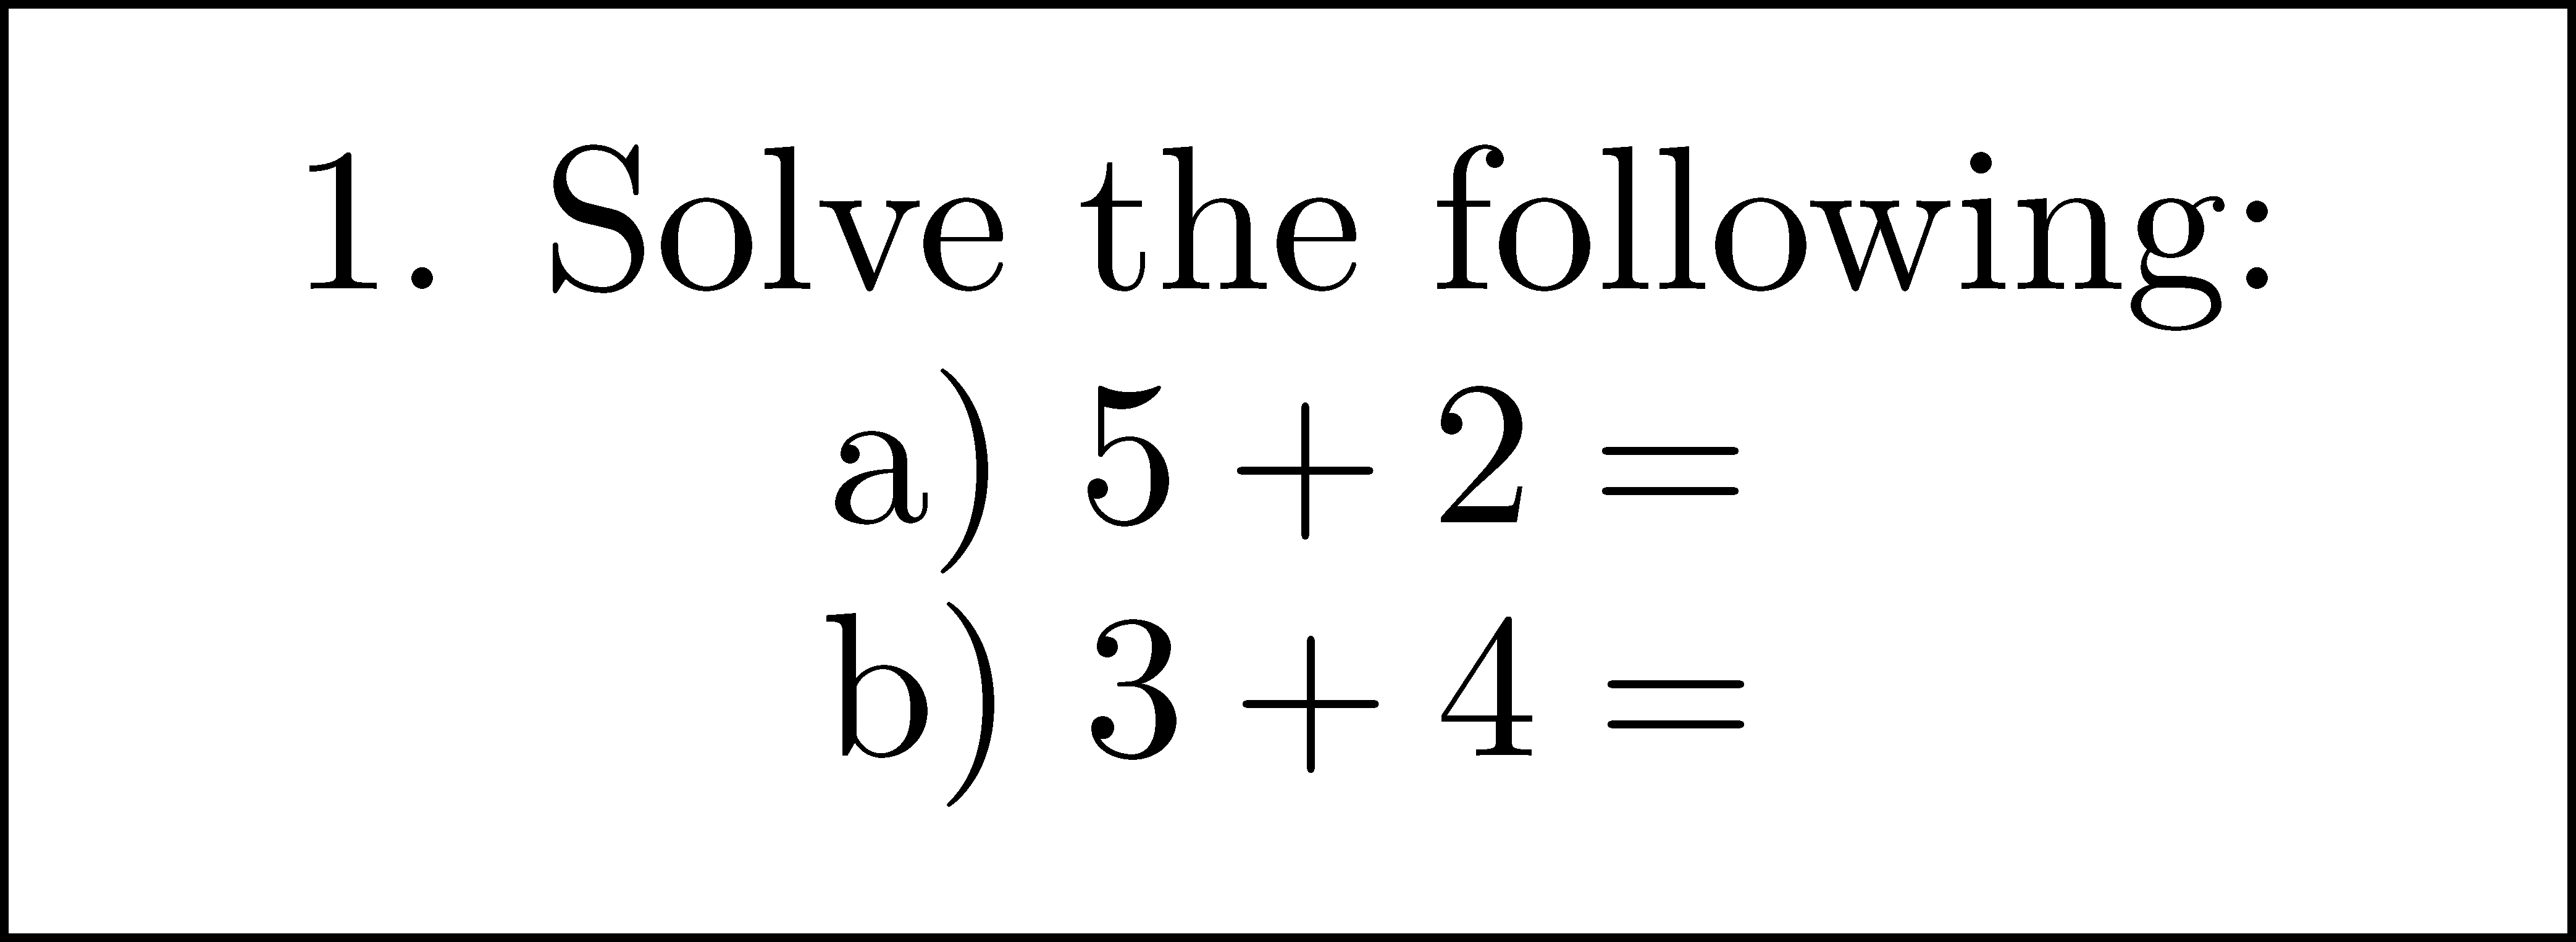
\includegraphics[width=0.35\linewidth]{tikz/sample_addition_problem} 

}

\caption{Sample problems}\label{fig:equality-operation}
\end{figure}

One of the common misconceptions surrounding the equal sign is that the symbol implies an action of doing some type of computation. For instance, students usually see the equal sign in the context of the type of problems seen in Figure @ref\{fig:equality-operation\}.

These type of problems promote an operational understanding of the equal sign, rather than a relational or substitutional understanding that is essential for later work \citep[pp.~145-150]{Cognition}. Because secondary mathematics students maintain many misconceptions about the concept of equality and the meaning of the equal sign, we will take some time to reflect on some key content standards from first grade that have a very strong influence on student success of learning mathematics in the middle school.

\begin{quote}
\hypertarget{related-content-standards-3}{%
\subsubsection*{Related Content Standards}\label{related-content-standards-3}}
\addcontentsline{toc}{subsubsection}{Related Content Standards}

\begin{itemize}
\tightlist
\item
  (1.OA.7) Understand the meaning of the equal sign, and determine if equations involving addition and subtraction are true or false. For example, which of the following equations are true and which are false? \(6 = 6\), \(7 = 8 - 1\), \(5 + 2 = 2 + 5\), \(4 + 1 = 5 + 2\).
\item
  (1.OA.8) Determine the unknown whole number in an addition or subtraction equation relating three whole numbers. For example, determine the unknown number that makes the equation true in each of the equations \(8 + ? = 11\), \(5 = ? - 3\), \(6 + 6 = ?\).
\end{itemize}
\end{quote}

\begin{figure}

{\centering \includegraphics[width=0.4\linewidth]{images/balance-scales} 

}

\caption{Pan balances}\label{fig:pan-balance}
\end{figure}

We should notice that in standard (1.OA.D.8) that the unknown should not always be at the end of a string of mathematical symbols and is based on educational research that compares students from different cultures and their understanding of the equal sign \citep[pp.~148-150]{Cognition}. Instead it should be at many different locations in order to make sure that students do not internalize the misconception that the equal sign means to compute. They should instead develop the concept of the equal sign representing two things that have the same value in some way. It is this understanding of two things looking different but representing the same underlying value that causes the equal sign to represent an equivalence.

Another method that may possibly contribute to a more relational understanding of the equal sign is the introduction of the equal sign alongside the greater than (\(>\)) and less than (\(<\)) symbols to emphasize the role of the equal sign in the comparison of the size of numbers. This comparison concept can be further reinforced with a pan balance (See Figure \ref{fig:pan-balance}).

This concept of a pan-balance can give students a concrete idea to attach to the meaning of the equal and inequality signs. However, like all good analogies, the pan balance is challenging to use with negative numbers and breaks down if you are comparing numbers in an unordered number system such as the complex numbers.

\hypertarget{exercises-8}{%
\subsection{Exercises}\label{exercises-8}}

A student is given the following task.

\begin{quote}
\begin{itemize}
\tightlist
\item
  Sophia goes to the store with \(\$5.00\) and buys two packs of gum for \(\$1.20\). She then gives \(\$2.00\) to her friend to buy a drink. How much money does she have left?
\end{itemize}
\end{quote}

\begin{enumerate}
\def\labelenumi{\arabic{enumi}.}
\item
  The student then writes the following on their paper.
  \[5.00-1.20=3.80-2.00=1.80, \mbox{ so Sophia has } \$1.80 \mbox{ left.}\]

  \begin{enumerate}
  \def\labelenumii{\alph{enumii}.}
  \item
    What ideas from this section regarding the equal sign and equivalence would you use to provide feedback to this student?
  \item
    What are other points of feedback that you would provide to this student?
  \end{enumerate}
\item
  If a student asks you what the equal sign means in the context of \(\frac{1}{2}=\frac{2}{4}\) since those symbols are not the same.
\item
  What are the meanings of the equal signs in the task?
  \textgreater Evaluate the function \(f(x)=3x-4\) for \(x=2\).
\end{enumerate}

\hypertarget{expressions-equations-and-inequalities}{%
\section{Expressions, Equations, and Inequalities}\label{expressions-equations-and-inequalities}}

A \textbf{numerical expression} is a meaningful string of numbers, operation symbols, and/or grouping symbols. In early elementary grades, examples of numerical expressions include \[2+6+4, \quad 13-3+2, \quad \mbox{ or } \quad (4+6)+3.\] In upper elementary grades, students are expected to incorporate rational numbers and the operations of multiplication, division, and exponents in order to be comfortable working with such expressions as
\[3 \times (10+4), \quad \frac{2}{3} \times (12+8), \quad \mbox{ or } \quad  2^3 + \frac{3+2}{7}.\]

In the transition from elementary school to secondary schools, students learn to add \textbf{variables}, symbols or letters that stand for any number within a specified range of numbers, to these expressions and thus work with \textbf{algebraic expressions} such as
\[100-10\cdot (P-15)^3,  \quad 3xy + 5(x-4)^2-7y^2, \quad 6\cdot (4x+3y), \quad \mbox{ or }\quad  \frac{3x+2}{2x-4}.\]

\begin{quote}
\hypertarget{related-content-standards-4}{%
\subsubsection*{Related Content Standards}\label{related-content-standards-4}}
\addcontentsline{toc}{subsubsection}{Related Content Standards}

\begin{itemize}
\tightlist
\item
  (6.EE.2) Write, read, and evaluate expressions in which letters stand for numbers.
\end{itemize}

\begin{enumerate}
\def\labelenumi{\alph{enumi}.}
\tightlist
\item
  Write expressions that record operations with numbers and with letters standing for numbers.
\item
  Identify parts of an expression using mathematical terms (sum, term, product, factor, quotient, coefficient); view one or more parts of an expression as a single entity.
\item
  Evaluate expressions at specific values of their variables. Include expressions that arise from formulas used in real-world problems. Perform arithmetic operations, including those involving whole-number exponents, in the conventional order when there are no parentheses to specify a particular order (Order of Operations).
\end{enumerate}
\end{quote}

In more advanced courses in secondary school mathematics, algebraic expressions can also include functions giving rise to expressions such as
\[f(x-h)+k, \quad \sin(3x)-2, \quad \mbox{ or } \quad  \ln(x+3).\]

The equivalence of numerical expressions is a key concept in the early elementary grades where students learn to compose and decompose numbers in different ways as they add and subtract numbers using different algorithms. In sixth grade, students are asked to determine the equivalence of two mathematical expressions. This definition that two algebraic expressions are equivalent if they generate the same number regardless of which number is substituted for the variable is one of the first places where students are pushed to move to the abstract realm of equivalence relations. We can verify that this definition of equivalent expressions is an equivalence relation using the fact that equality on the real numbers is an equivalence relation.

\begin{quote}
\hypertarget{related-content-standards-5}{%
\subsubsection*{Related Content Standards}\label{related-content-standards-5}}
\addcontentsline{toc}{subsubsection}{Related Content Standards}

\begin{itemize}
\tightlist
\item
  (6.EE.3) Apply the properties of operations to generate equivalent expressions. \%\{\em For example, apply the distributive property to the expression $3 (2 + x)$ to produce the equivalent expression $6 + 3x$; apply the distributive property to the expression $24x + 18y$ to produce the equivalent expression $6 (4x + 3y)$; apply properties of operations to $y + y + y$ to produce the equivalent expression $3y$.\}
\item
  (6.EE.4) Identify when two expressions are equivalent (i.e., when the two expressions name the same number regardless of which value is substituted into them).
\item
  (6.EE.5) Understand solving an equation or inequality as a process of answering a question: which values from a specified set, if any, make the equation or inequality true? Use substitution to determine whether a given number in a specified set makes an equation or inequality true.
\end{itemize}
\end{quote}

While substituting in values to determine if two expressions are equivalent is the definition of the equivalence, it is almost always impossible to substitute in all possible values for a variable, as there are infinitely many possibilities in most situations. Instead, we determine the equivalency of two expressions by applying various properties of the operations. For example, the distributive property shows us that \(3(x+y)\) is equivalent to \(3x+3y\). However, students have to be careful to consider the set of possible numbers for an expression when determining the equivalence of \(\sqrt{x^2}\) and \(x\), or \(\frac{3x^2}{x}\) and \(3x\).

An \textbf{equation} is a statement that a number or expression is equivalent to a different number or expression. An equation that is true for all values of the variable is called an \textbf{identity}. The associative, commutative, and distributive properties of the number systems
\begin{align*}
    a+(b+c) &= (a+b)+c \\
    a+b &= b+a \\
    a \times (b+c) &= (a\times b)+(a\times c)
\end{align*}
are all common identities. Some other common identities in this regard are the trigonometric identity
\begin{align*}
    \cos^2(\theta) + \sin^2(\theta) &= 1  \\
    \sin(\alpha \pm \beta) &= \sin(\alpha)\cos(\beta)\pm \cos(\alpha)\sin(\beta) \\
    \cos(2\theta) &= \cos^2(\theta)-\sin^2(\theta)
\end{align*}
that are used to simplify trigonometric expressions.

An equation that describes how multiple quantities vary together is usually called a \textbf{formula}. These can include the area formula for rectangles defined by \(\mbox{Area}=\mbox{width} \times \mbox{height}\) or Boyle's law where pressure (\(P\)) is inversely proportional to volume (\(V\)), i.e.~\(PV =k\) for some constant \(k\).

While the identity equations hold true irrespective of the values of the variables, it is often the case that equations hold for only some of the possible values for the variables, or possibly even none. We can then \textbf{solve} such equations by determining which values, called \textbf{solutions to the equation}, for the variables cause the equation to be a true statement.

Similar to equations, \textbf{inequalities} are statements that a number or expression is related to a different number or expression in a certain order relation. Some of these inequalities are identities or formulas, such as \(x\leq |x|, x\in\mathbb{R}\), while some have a solution set, such as \(x^2+y^2<1\).

\begin{definition}
\protect\hypertarget{def:unnamed-chunk-48}{}{\label{def:unnamed-chunk-48} } Two equations (inequalities) are equivalent if they are true statements for the same values of the variables.
\end{definition}

In the process of finding solutions to equations or inequalities, it is almost always helpful to rewrite an equation or inequality as an equivalent equation or inequality. For instance in an effort to find the solutions to \[\frac{x^2-10x+21}{3x-12} = \frac{x-5}{x-4}\]
we want to find an expression that is equivalent to the left side of the equation. Such an expression could be \[\frac{(x-3)(x-7)}{3(x-4)},\] with the equivalency of the expressions verified using the distributive property. Since these two expressions are equivalent, they have the same values for every value of the variable. This means that the original equation is a true statement if, and only if, \[\frac{(x-3)(x-7)}{3(x-4)}=\frac{x-5}{x-4}\] is a true statement. We also know that if two numbers are the same, then \(3\) times each of the numbers are also the same. So the original statement is true if, and only if, the equivalent equation
\[\frac{(x-3)(x-7)}{x-4}=\frac{3(x-5)}{x-4}\] is true. If \(x=4\), then the statement would have no meaning, as division by zero has no meaning. This means that we can eliminate \(4\) from the set of possible solutions. With \(x\neq 4\) we can multiply both sides of the equation by \((x-4)\) to generate the equivalent equation, \[(x-3)(x-7)=3(x-5).\] We can use the distributive property again to create an equivalent equation of \[x^2-10x+21=3x-15.\] Since we can also add the same expression, \(-3x+15\), to both sides of the equation and create an equivalent equation, we see that the original equation is equivalent to \[x^2-13x+36=0\] as long as \(x\neq 4\). Using the distributive property, we see that this equation is equivalent to \[(x-4)(x-9)=0.\] So the original equation is a true statement if, and only if, \((x-4)(x-9)=0\) is a true statement and \(x\neq 4\). This only occurs when the variable, \(x\), is equal to \(9\).

Through this process we can see how equivalence of equations is essential in the process of finding solutions to equations. This means that as students make the transition from elementary to secondary, it is important for teachers to be understanding of the challenge of thinking about equivalent expressions and to be explicit about this relationship.

\hypertarget{exercises-9}{%
\subsection{Exercises}\label{exercises-9}}

\begin{enumerate}
\def\labelenumi{\arabic{enumi}.}
\tightlist
\item
  Most of this project will be in the context of algebraic reasoning and these questions should be answered with the expectations of your target student population.

  \begin{enumerate}
  \def\labelenumii{\alph{enumii}.}
  \tightlist
  \item
    What is the difference between an expression and equation?
  \item
    Why can we not solve an expression?
  \item
    What does it mean to ``solve an equation''?
  \item
    What makes two expressions equivalent to each other?
  \item
    What is the difference between how the equality sign is used when solving an equation versus when working with expressions?
  \end{enumerate}
\item
  Prove that the definition of equivalent equations forms an equivalency relation.
\end{enumerate}

\hypertarget{ch:number}{%
\chapter{Number Systems}\label{ch:number}}

K-12 mathematics is rich in the study of number systems, with particular focus on the Natural Numbers, Integers, Rational Numbers, Real Numbers, and Complex Numbers. In this chapter we use the properties of set theory and equivalence classes discussed in Chapters \ref{ch:sets} and \ref{ch:equivalence} to construct these numbers systems. We follow this discussion with a study of some of the properties of number systems, connecting them to the K-12 curriculum. Lastly, we examine different representations of these number systems helpful for developing numerical fluency and conceptual understanding of the numerical operations.

This process of constructing the number systems is very abstract and challenging for those who have not previously studied these constructions. The process is included because it helps teachers to better understand the abstract nature of the number systems and some of the challenges of their students. While working with many of these number systems has become second nature for math teachers, the initial learning by students is much harder than expected for new teachers and so a deeper knowledge of the properties of the number system helps in this teaching situation.

\[\mathbb{N} \subseteq \mathbb{Z} \subseteq \mathbb{Q} \subseteq \mathbb{R} \subseteq \mathbb{C}\]
As we are working with the various number systems, we will use varying notation for our operations. With all of the constructions, subtraction and division are not defined. We instead define the additive inverse and multiplicative inverse and so we can think of subtraction \(a-b\) as \(a+(-b)\) and division \(a\div b\) as \(a \times \frac{1}{b}\). We will also use various symbols to represent multiplication so that \(a\times b\), \(a\cdot b\), and \(ab\) all represent the same thing.

\hypertarget{sec:Integers}{%
\section{Natural Numbers and Integers}\label{sec:Integers}}

As part of the effort to axiomatize mathematics in the late 19\textsuperscript{th} and early 20\textsuperscript{th} centuries, individuals such as Richard Dedekind (1831-1916), Georg Cantor (1845-1918), Giuseppe Peano (1858-1932), Alfred Whitehead (1861-1947), David Hilbert (1862-1943), Ernst Zermelo (1871-1953), Bertrand Russell (1872-1970), and Abraham Fraenkel (1891-1965) followed a program to start with the most basic of assumptions and build a solid foundation for the field of mathematics. One of the greatest works in this program is the \emph{Principia Mathematica} by Whitehead and Russell \citetext{\citeyear{Principia1}; \citeyear{Principia2}; \citeyear{Principia3}} that built such a foundation on logic and set theory that it took until page 86 of the second volume to prove that \(1+1=2\). While we will not go to the full extent of abstraction, we will build up the natural numbers and the integers from the axioms of Zermelo-Fraenkel set theory, together with the axiom of choice (ZFC axioms).

\hypertarget{natural-numbers}{%
\subsection{Natural Numbers}\label{natural-numbers}}

We will study the concepts of counting and related ideas of the natural numbers in Chapter \ref{ch:function}, but initially we will use John von Neumann's \citeyearpar{vonNeumann23} definition for the natural numbers which are defined inductively by defining the symbols
\[0:=\emptyset, \quad 1:=\{\emptyset\}, \quad 2:=\{\emptyset, \{\emptyset\}\},\] and so on. So for any natural number \(n\), the next natural number is defined inductively as \[n+1:=S(n) := n\cup \{n\},\] where you think of \(S(n)\) as the successor of \(n\).

This definition of the natural numbers is highly dependent upon the axiom of infinity from the ZFC axioms. In the formal language of the ZFC axioms, the axiom of infinity is stated as
\[\exists I ( \emptyset\in I \wedge \forall x\in I((x\cup \{x\})\in I).\] Or equivalently, there is a set \(I\) that contains the empty set as an element and that if \(x\in I\), then \(x\cup \{x\}\) is also in \(I\). The set \(I\) is a larger set than \(\mathbb{N}\), but allows for the existence of the natural numbers.

With our definition of the natural numbers, we also have that \(S(n)\neq n\), \[S(n)=S(m) \Leftrightarrow n=m,\] and we can create an order on the set of symbols \(\mathbb{N} = \{0, 1, 2, 3, \ldots \}\) by defining that
\[n \leq m \Longleftrightarrow n \subseteq m.\] One can prove that this set of symbols satisfies the well-ordering property (@ref(def:well\_ordering)) using the ZFC axioms, which enables us to prove the principle of mathematical induction creating the mathematical machinery necessary for the study of the natural numbers.

\begin{theorem}[Principle of Mathematical Induction]
\protect\hypertarget{thm:unnamed-chunk-49}{}{\label{thm:unnamed-chunk-49} \iffalse (Principle of Mathematical Induction) \fi{} }Suppose that \(S\) is a subset of \(\mathbb{N}\) such that \(0\in S\), and for all \(n\in \mathbb{N}\), \(n\in S\) implies that \(S(n) \in S\).

Then \(S\) must be the set of natural numbers.
\end{theorem}

We will leave the detailed proof for a text on symbolic logic. However, the application of this theorem is that if we have a mathematical statement that varies along the natural numbers, \(P(n)\). If the statement \(P(0)\) is true, and if \(P(k)\) being true implies that \(P(k+1)\) is true, then \(P(n)\) must be true for all natural numbers.

We inductively define the operation of addition on these symbols so that for any integer \(a\),
\begin{align*}
    a+0 &:=a, \\
    a+1 := a+S(0) &= S(a+0), \\
    a+2:=a+S(1) &= S(a+1), \\
    \vdots \\
    a+S(b) &:= S(a+b)
\end{align*}
We similarly define multiplication inductively by
\[a\times 0 := 0, \quad a\times 1 := (a \times 0)+a = a, \quad \mbox{ and } \quad a\times S(b) := (a\times b)+a.\]
With these operations we have the following properties of the natural numbers.

\begin{theorem}
\protect\hypertarget{thm:unnamed-chunk-50}{}{\label{thm:unnamed-chunk-50} }Let \(a\), \(b\), and \(c\) be natural numbers. Then

\begin{itemize}
\tightlist
\item
  \(a+b\) and \(a\times b\) are natural numbers (closure)
\item
  \(a+(b+c)=(a+b)+c\) and \(a\times (b\times c)=(a\times b)\times c\) (associative property)
\item
  \(a+b=b+a\) and \(a\times b=b\times a\) (commutative property)
\item
  \(a+0=a\) and \(a\times 1 =a\) (additive and multiplicative identities)
\item
  \(a \times (b+c)= (a\times b) + (a\times c)\) (distributive property)
\item
  If \(a\times b=0\), then \(a=0\) or \(b=0\) (or both). (no non-zero divisors)
\end{itemize}
\end{theorem}

In order to get a flavor for the techniques involved in proving these properties, we will prove the associative property of addition for the natural numbers. The proofs of the remainder of the statements will be left to the reader to work through.
\begin{proof}
\iffalse{} {Proof. } \fi{}Let \(a,b \in \mathbb{N}\). Then, for each \(c\in \mathbb{N}\), we let \(P(c)\) be the statement that
\[a+(b+c) = (a+b) + c.\]

If \(c=0\), then \(b+c=b\) and \((a+b)+c=a+b\), and so
\[a+(b+c)=a+b= (a+b)+c.\] This implies that \(P(0)\) is true.

Assume by that for some value of \(c'\in \mathbb{N}\) that \(P(c')\) is true, i.e.~that \(a+(b+c')=(a+b)+c'\) (\(c'=0\) is true and so such a \(c'\) exists). Then for \(c=S(c')\),
\begin{align*}
    a+(b+c) &= a+(b+S(c'))=a+S(b+c') \\
    &= S(a+(b+c')) = S((a+b)+c') \: \mbox{ (by the induction hypothesis)}\\
    &= (a+b)+S(c') = (a+b)+c.
\end{align*}

Therefore, P(c) is true. and by the principle of mathematical induction we have that \(a+(b+c)=(a+b)+c\) for all values of \(a,b,c\in \mathbb{N}\).
\end{proof}

We previously defined the order on the natural numbers using set inclusions. This order can be rewritten using operations by noting that \(m<n\) if, and only if, \(n=m+k\) for some natural number \(k\). We will explore how this order interacts with the operations of addition and multiplication.

\begin{lemma}
\protect\hypertarget{lem:order-addition-naturals}{}{\label{lem:order-addition-naturals} }Let \(m,n,k\in \mathbb{N}\). Then \[ (1) \: (m=n) \Leftrightarrow (m+k=n+k) \quad \mbox{ and } \quad (2) \: (m<n) \Leftrightarrow (m+k<n+k).\]
\end{lemma}

\begin{proof}
\iffalse{} {Proof. } \fi{}We will prove part \((1)\) using an induction argument on \(k\) using the statement that given \(m,n\in \mathbb{N}\), \(P(k)\) is the statement that \((m=n) \Leftrightarrow (m+k=n+k)\). Since \(0\) is the additive identity, we know that \(P(0)\) is true. We also have from the definition of \(S(n)\) that \(P(1)\) is true. If we assume for some \(l\in \mathbb{N}\) that \(P(l)\) is true, then \(m+(l+1) = n+(l+1)\) is equivalent to \((m+l)+1 = (n+l)+1\), and since \(P(1)\) is true this is equivalent to \((m+l)=(n+l)\). So \(P(l)\) being true implies that \(P(l+1)\) is true. Therefore, \(P(k)\) is true for all \(k\in \mathbb{N}\).

In order to prove part \((2)\), we note that
\begin{align*}
    (m<n) &\Leftrightarrow (\mbox{There exists } j\in \mathbb{N} \mbox{ such that } (n=m+j)) \\
    &\Leftrightarrow (\mbox{There exists } j\in \mathbb{N} \mbox{ such that } ((n+k)=(m+j)+k)) \\
    &\Leftrightarrow (\mbox{There exists } j\in \mathbb{N} \mbox{ such that } ((n+k)=(m+k)+j)) \\
    &\Leftrightarrow (m+k<n+k).        
\end{align*}
\end{proof}

\begin{lemma}
\protect\hypertarget{lem:order-multiplication-naturals}{}{\label{lem:order-multiplication-naturals} }Let \(m,n,k\in \mathbb{N}\). Then \[ (1) \: (m=n) \Leftrightarrow (m\times k=n\times k) \quad \mbox{ and } \quad (2) \: (m<n) \Leftrightarrow (m\times k<n\times k), \mbox{ for } k>0.\]
\end{lemma}

The proof of this lemma is very similar to the previous lemma and is left as an exercise.

\hypertarget{integers}{%
\subsection{Integers}\label{integers}}

Now that we have defined the set of the natural numbers (\(\mathbb{N}\)) and the operations on \(\mathbb{N}\) of addition and multiplication, we would like to have additive inverses. However, we do not assume that the set of additive inverses exist, but instead construct the integers from the natural numbers.

Subsection \ref{subsec:cartesian} gives the existence of the set \[\mathbb{N}\times \mathbb{N} = \{ (a,b)  \vert a,b \in \mathbb{N}\}.\] On this set of ordered pairs, we will define an equivalence relation that
\[(a,b)\sim (c,d) \quad \Leftrightarrow \quad  a+d=b+c.\]

Since this is an equivalence relation we can define \(\mathbb{Z}\) to be the set of equivalence classes under this relation. We will denote by \([(a,b)]\) the equivalence class containing \((a,b)\).

We can now define the operations of addition and multiplication on this set of equivalence classes.
\[[(a,b)]+[(c,d)]:= [(a+c,b+d)] \quad \mbox{and} \quad [(a,b)]\times [(c,d)] := [(ac+bd,ad+bc)]\]

We need to make sure that these definitions are well-defined in that the operations do not depend on which element of the equivalence class is chosen for the representation. Assume that \((a,b)\) and \((a',b')\) are both elements of \([(a,b)]\) and that \((c,d)\) and \((c',d')\) are both elements of \([(c,d)]\). This is equivalent to the statements that \[a+b'=b+a' \quad \mbox{ and } c+d'=d+c'.\] So, using properties of equivalent equations involving natural numbers we can add the two equations together and see that \[(a+b') + (c+d') = (b+a')+(d+c').\] Using the associative and commutative properties of addition for the natural numbers we see that this equation is equivalent to \[(a+c) + (b'+d') = (b+d) + (a'+c')\] and so \([(a+c,b+d)]\) is equivalent to \([(a'+c',b'+d')]\), proving that addition is well-defined. The proof that multiplication is well-defined is left as an exercise.

We can also put an order on this set by defining that \[[(a,b)] < [(c,d)] \Leftrightarrow a+d<b+c.\]

We can think of the natural numbers, \(\mathbb{N}\), as the subset of \(\mathbb{N}\times \mathbb{N}\) of the form
\[\mathbb{N} := \mathbb{N} \times \{0\} = \{ [(a,0)] \vert a\in \mathbb{N}\},\] since \([(a,0)]+[(b,0)] = [(a+b,0)]\) and \([(a,0)] \times [(b,0)] = [(ab,0)]\).

With this identification of the natural numbers with \(\mathbb{N}\times \{0\}\), where \(a=[(a,0)]\), we are able to see that the negative integers can be associated with \(\{0\} \times \mathbb{N}\), since \([(a,0)]+[(0,a)] = [(a,a)] = [(0,0)]\). We then label \([(0,a)]\) as \$ - {[}(a,0){]}\$, and usually write it as \(-a\). We can then identify every element of \(\mathbb{N}\times \mathbb{N}\) with an integer,
\[[(a,b)] \leftrightarrow a+(-b).\]

Thus we have constructed a new set \(\mathbb{Z}\) with the operations of addition and multiplication that satisfy the properties for \(a,b,c\in \mathbb{Z}\) in Table \ref{tab:intprops}.

\begin{table}

\caption{\label{tab:intprops}Properties of Integers}
\centering
\begin{tabular}[t]{l|l|l}
\hline
 &  & Property\\
\hline
\$a+b\$ is an integer & \$a \textbackslash{}times b\$ is an integer & Closure\\
\hline
\$a+(b+c)  = (a+b)+c\$ & \$a \textbackslash{}times (b \textbackslash{}times c) = (a \textbackslash{}times b) \textbackslash{}times c\$ & Associative Property\\
\hline
\$a+b=b+a\$ & \$a\textbackslash{}times b = b\textbackslash{}times a\$ & Commutative Property\\
\hline
\$a+0=a\$ & \$a \textbackslash{}times 1 = a\$ & Additive and Multiplicative Identities\\
\hline
\$a \textbackslash{}times (b+c) = (a\textbackslash{}times b) + (a \textbackslash{}times c)\$ & \$(a+b) \textbackslash{}times c = (a\textbackslash{}times c) + (b\textbackslash{}times c)\$ & Distributive Property\\
\hline
\$a + (-a) =0\$ &  & Additive Inverses\\
\hline
If \$a,b>0\$, then \$ab>0\$. & If \$a,b<0\$, then \$ab>0\$. & \$ab<0\$ if, and only if,  \$a\$ and \$b\$ are opposite signs.\\
\hline
\$ab=0\$ if, and only if, \$a=0\$, \$b=0\$, or both &  & No zero divisors\\
\hline
\end{tabular}
\end{table}

While the integers do not satisfy the Well-Ordering Property (\ref{def:well-ordering}), since the negative numbers are a non-empty set without a least element, it does satisfy the least-upper-bound property that any non-empty set that is bounded above has a least upper bound.

The integers do however, have generalizations of Lemmas \ref{lem:order-addition-naturals} and \ref{lem:order-multiplication-naturals}, with the proofs following directly from various properties listed in Table \ref{tab:intprops}.

\begin{theorem}
\protect\hypertarget{thm:unnamed-chunk-53}{}{\label{thm:unnamed-chunk-53} }Let \(m,n,k\in \mathbb{Z}\). Then \[(1) \: (m=n) \Leftrightarrow (m+k=n+k),  \quad (2) \: (m<n) \Leftrightarrow (m+k<n+k),\]
\[ (3) \: (m=n) \Leftrightarrow (m\times k=n\times k), \mbox{ with } k\neq 0 \quad \mbox{ and } \quad (4) \: (m<n) \Leftrightarrow (m\times k<n\times k), \mbox{ with } k> 0 .\]
\end{theorem}

\hypertarget{properties-of-exponents}{%
\subsection{Properties of Exponents}\label{properties-of-exponents}}

Let \(a\) be an integer. We define \(a^n\) for each natural number \(n\) using the following recursive definition.
\[a^0:=1, \quad a^1 := a, \quad \mbox{ and } \quad a^{n+1}:=a \cdot a^n\, \: \forall n\in \mathbb{N}.\]

Notice that we have defined \(0^0=1\). This is not a universally accepted definition, but is widely accepted in the context of algebraic and combinatoric contexts, while left as indeterminate in a limit context of analysis, since
\[\lim_{x\rightarrow 0^+} x^0 = 1 \quad \mbox{ and } \quad \lim_{x\rightarrow 0^+} 0^x = 0.\]

\begin{quote}
\hypertarget{related-content-standards-6}{%
\subsubsection*{Related Content Standards}\label{related-content-standards-6}}
\addcontentsline{toc}{subsubsection}{Related Content Standards}

\begin{itemize}
\tightlist
\item
  (6.EE.1){]} Write and evaluate numerical expressions involving whole-number exponents.
\end{itemize}
\end{quote}

With this definition, we are able to prove many of the properties of exponents of natural numbers with a base of an integer. It is already given that \(a^0=1\) and \(a^1=a\).

\begin{lemma}
\protect\hypertarget{lem:exponent-addition}{}{\label{lem:exponent-addition} }Let \(a\) be an integer, and let \(m\) and \(n\) be natural numbers. Then
\[a^m\cdot a^n=a^{m+n}.\]
\end{lemma}

\begin{proof}
\iffalse{} {Proof. } \fi{}That we are trying to prove something to be true for all natural numbers points us to a proof by induction argument. In this case, we will fix \(n\in \mathbb{N}\) and let \(P(m)\) be the statement that \(a^m\cdot a^n=a^{m+n}\).

Then \(P(0)\) is the statement that \(a^0\cdot a^n = a^{0+n}\). Since \(a^0=1\) and \(0+n=n\), we have that \(1\cdot a^n = a^n\), which is a true statement.

If we assume that \(P(k)\) is true for some value of \(k\) (we already know that it is true for \(k=0\)), then \(a^k\cdot a^n = a^{k+n}\). This means that
\begin{align*}
    a^{(k+1)} \cdot a^n & = (a \cdot a^k) \cdot a^n \mbox{ (by the definition of the exponent)} \\
    &= a \cdot (a^k\cdot a^n) \mbox{ (since multiplication is associative for integers)} \\
    &= a \cdot a^{k+n} \mbox{ (by the assumption that $P(k)$ is true)} \\
    &= a^{(k+n+1)} \mbox{ (by the definition of the exponent)} \\
    &= a^{(k+1)+n} \mbox{ (since addition is associative for the natural numbers)}.
\end{align*}
So, \(P(k+1)\) is true.

Therefore, by induction, \(P(m)\) is true for all natural numbers \(m\).
\end{proof}

\begin{lemma}
\protect\hypertarget{lem:unnamed-chunk-55}{}{\label{lem:unnamed-chunk-55} }Let \(a\) and \(b\) be any integers, and let \(n\) be any natural number. Then \[(ab)^n=a^n \cdot b^n.\]
\end{lemma}

\begin{proof}
\iffalse{} {Proof. } \fi{}Since we are proving a statement to be true for all natural numbers, we will use a proof by induction with the statement \(P(n)\) being that \((ab)^n=a^n\cdot b^n\).

Since \(P(0)\) is the statement that \((ab)^0=a^0 \cdot b^0\), we have that this is equivalent to the statement that \(1=1\), and so is true.

If we assume that \(P(k)\) is true for some value of \(k\), then we have that \((ab)^k=a^k\cdot b^k\). We can then use properties of addition and multiplication of integers, and the definition of exponents, to see that \[(ab)^{(k+1)}= (ab)^k\cdot (ab) = a\cdot (ab)^k \cdot b = (a\cdot a^k) \cdot (b^k\cdot b)  = a^{(k+1)} \cdot b^{(k+1)}\] and so \(P(k+1)\) is true.

Therefore, by induction, \(P(n)\) is true for all \(n\in \mathbb{N}\).
\end{proof}

\begin{lemma}
\protect\hypertarget{lem:exponent-product}{}{\label{lem:exponent-product} }Let \(a\) be an integer and \(n\) and \(m\) be any natural numbers. Then \[(a^m)^n = a^{mn}.\]
\end{lemma}

The proof of this lemma is similar to the proof of Lemma \ref{lem:exponent-addition} and so will be left as an exercise.

\begin{lemma}
\protect\hypertarget{lem:unnamed-chunk-57}{}{\label{lem:unnamed-chunk-57} }Let \(a\) and \(b\) be integers with \(0<a<b\). Then for each natural number \(n\geq 1\), \(0<a^n<b^n\).
\end{lemma}

\begin{proof}
\iffalse{} {Proof. } \fi{}We will use an induction argument for fixed integers \(a\) and \(b\), with \(a<b\). We let \(P(n)\) be the statement, \(0<a^n<b^n\). Since \(a^1=a\) and \(b^1=b\), we see that \(P(1)\) is true. If for some \(k\in \mathbb{N}\), with \(k\geq 1\), \(P(k)\) is true, then
\[ a^{(k+1)}=a^k\cdot a^1 < b^k \cdot a^1 < b^k \cdot b^1 = b^{(k+1)}\] using the induction hypothesis and Lemma \ref{lem:order-multiplication-naturals}. Since the natural numbers are closed under multiplication, and therefore also under exponents, we have that \(P(k+1)\) is true. Therefore, \(P(n)\) is true for all \(n\in \mathbb{N}\), with \(n\geq 1\).
\end{proof}

We will summarize these results in the following theorem and extend these properties to other number systems throughout the remainder of the chapter.

\begin{theorem}
\protect\hypertarget{thm:exponents-integers}{}{\label{thm:exponents-integers} }Let \(a\) and \(b\) be integers.

\begin{enumerate}
\def\labelenumi{\alph{enumi}.}
\item
  \(a^0=1\)
\item
  \(a^1=a\)
\item
  \(a^m\cdot a^n = a^{m+n}\) for each \(m,n\in \mathbb{N}\)
\item
  \((ab)^n=a^n\cdot b^n\) for each \(n\in \mathbb{N}\)
\item
  \((a^m)^n = a^{mn}\) for each \(m,n\in \mathbb{N}\)
\item
  If \(0<a<b\), \(0<a^n<b^n\) for each \(n\in \mathbb{N}\)
\end{enumerate}
\end{theorem}

\hypertarget{exercises-10}{%
\subsection{Exercises}\label{exercises-10}}

\begin{enumerate}
\def\labelenumi{\arabic{enumi}.}
\item
  After introducing the associative property for addition, a student asks if there is something similar for subtraction so that
  \[ A-(B-C) = (A-B)-C.\] How would you respond to the student?
\item
  Prove that the relation on \(\mathbb{N}\times\mathbb{N}\) defined by \[(a,b)\sim (c,d) \quad \Leftrightarrow \quad a+d=b+c\] is an equivalence relation.
\item
  Prove Lemma \ref{lem:order-multiplication-naturals}.
\item
  Prove Lemma \ref(lem:exponent-product).
\end{enumerate}

\hypertarget{sec:integer-representation}{%
\section{Representations of Integers}\label{sec:integer-representation}}

\hypertarget{sec:rationals}{%
\section{Rational Numbers}\label{sec:rationals}}

\hypertarget{representations-of-rational-numbers}{%
\section{Representations of Rational Numbers}\label{representations-of-rational-numbers}}

\hypertarget{sec:reals}{%
\section{Real Numbers}\label{sec:reals}}

\hypertarget{sec:complex}{%
\section{Complex Numbers}\label{sec:complex}}

\hypertarget{ch:function}{%
\chapter{Functions}\label{ch:function}}

\hypertarget{part-algebra}{%
\part{ALGEBRA}\label{part-algebra}}

\hypertarget{ch:group-1}{%
\chapter{Groups, Rings, and Fields}\label{ch:group-1}}

\hypertarget{ch:rings}{%
\chapter{Integral Domains and Polynomials}\label{ch:rings}}

\hypertarget{ch:real-valued-functions}{%
\chapter{Real Valued Functions}\label{ch:real-valued-functions}}

\hypertarget{part-geometry}{%
\part{GEOMETRY}\label{part-geometry}}

\hypertarget{ch:constructions}{%
\chapter{Axiomatic Geometry}\label{ch:constructions}}

\hypertarget{ch:measurement}{%
\chapter{Measurement}\label{ch:measurement}}

\hypertarget{ch:algebraic-geometry}{%
\chapter{Groups and Geometry}\label{ch:algebraic-geometry}}

\hypertarget{ch:transformations}{%
\chapter{Euclidean Transformational Geometry}\label{ch:transformations}}

\hypertarget{part-data-analysis}{%
\part{DATA ANALYSIS}\label{part-data-analysis}}

\hypertarget{ch:data1}{%
\chapter{Data Analysis Foundations}\label{ch:data1}}

\hypertarget{ch:data-explore}{%
\chapter{Exploring Data}\label{ch:data-explore}}

\hypertarget{ch:simulations}{%
\chapter{Samples, Simulations, and Probability}\label{ch:simulations}}

\hypertarget{ch:parameters}{%
\chapter{Estimating Parameters and Testing Hypotheses}\label{ch:parameters}}

  \bibliography{mkt.bib}

\end{document}
